\documentclass[fleqn]{beamer}
 
 
\usepackage{dsfont}
\usepackage[utf8]{inputenc} 
\usepackage[T1]{fontenc}
\usepackage{lmodern}
\usepackage{graphicx}
\usepackage{units}
\usepackage{amsmath}
\usepackage{array}
\usepackage{textcomp}
\usepackage{biblatex}
\usepackage{stmaryrd} 
\usepackage{enumerate}
\usepackage{amsmath}
\usepackage{amsthm}
\usepackage{mathrsfs}
\usepackage{relsize}

\usetheme{CambridgeUS}

\newcommand\norm[1]{\left\lVert#1\right\rVert}

\setbeamertemplate{itemize subitem}[triangle] 
\setbeamertemplate{itemize subsubitem}[circle]
 
\begin{document}
\title{Automatic Calibration of Large Traffic Models}
\date{August $27^{th}$, 2015}
\author[Meziere, Gomes]{Felix Meziere \thanks{Ecole polytechnique [felix.meziere@polytechnique.edu]} \and Gabriel Gomes \thanks{University of California Berkeley [gomes@path.berkeley.edu]}}
\institute[PATH]{California PATH Program}
\maketitle
 
\begin{frame}
\frametitle{Introduction}
\framesubtitle{and motivation of this work}
\begin{itemize}
	\item Calibrate large traffic models input:
	\begin{itemize}
		\item Constants of the scenario
		\item Source and sink flows depending on day of week \& moment of year
	\end{itemize}	
	\item for the output to match:
	\begin{itemize}
		\item Congestion
		\item VMT and VHT
		\item Credible ramp flows
	\end{itemize}
	\item Goal: model accurately a usual traffic situation to make predictions.
\end{itemize}
\end{frame}

\begin{frame}
	\frametitle{Setup}
	\framesubtitle{Freeway and traffic model, data, notation}
	\begin{center}
		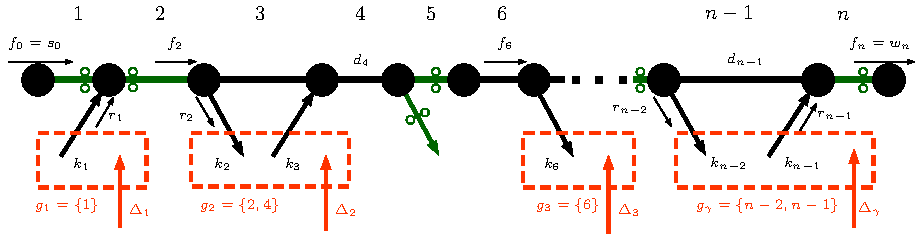
\includegraphics[width=4.5in]{figures/presentation_scheme.pdf}
	\end{center}
	\scriptsize{\begin{tabular}{llll}
		$M=\llbracket 1,n \rrbracket$ & Mainline link indexes  & $(f_{i}(t))_{i\in{M}}$ & Mainline links exit flows\\
		$R\subset{M}$ & Ramp link indexes & $(d_{i}(t))_{i\in{M}}$ & Mainline links densities\\
		$T\subset{M}$ & Monitored mainline links & $(r_{i}(t))_{i\in{R}}$ & Ramps exit flows\\
		$K\subset{R}$ & Non-Monitored ramps & $(\widetilde{f}_{i}(t))_{i\in{T}}$ & Measured mainline exit flows\\
		$G=(g_{i})_{i\in{\llbracket 1,\gamma \rrbracket}}$ & Knob group indexes  & $(\widetilde{d}_{i}(t))_{i\in{T}}$ & Measured mainline densities\\
		$\vec{k}=(k_{i_{1}},k_{i_{2}}...,k_{i_{\kappa}})$ & Knobs value vector  & $(\widetilde{r}_{i}(t))_{i\in{(R\backslash K)}}$ & Measured ramps exit flows\\
		$\sigma=(\sigma_{i_{1}},\sigma_{i_{2}}...,\sigma_{i_{\kappa}})$ & on/off-ramp indicator & $\tau$, $D$ & Set of time-steps, Duration\\
		
	\end{tabular}} 
\end{frame}

%\begin{frame}
%	\frametitle{Setup}
%	\framesubtitle{Context : PeMS data for 210E}
%	\begin{itemize}
%	\item Average of 5 Tuesdays in fall 2014
%	\item Flow, density and speed on 74 links every 5 minutes for 24 hours
%	\item Sensors (having deleted partial or too biased):
%	\begin{itemize}
%	\item 33/135 Mainline links are monitored
%	\item 26/28 On-ramps are monitored
%	\item 15/25 Off-ramps are monitored
%	\end{itemize}
%	\item Assumptions : uncertainty from sensor sensibility and bias
%	\begin{itemize}
%	\item Daily local flow uncertainty on mainline sensors : $I^{local}\approx10\%.[Average\ of\ mainline\ flow]$
%	\item Daily global uncertainty (on measures summed over the whole freeway): $I^{global}\approx5\%.[Global\ measure\ value]$
%	\end{itemize}
%	\end{itemize}
%\end{frame}

%\begin{frame}
%\frametitle{Setup}
%\framesubtitle{BeATS}
%Macroscopic freeway simulator
%\begin{itemize}
%\item Input:
%\begin{itemize}
%\item Topography of the freeway
%\item Fundamental Diagrams
%\item 5-min demands for sources and sinks ("split-ratios as output mode")
%\begin{itemize}
%\item As real data if the source or sink is monitored
%\item As a guessed template if not $\rightarrow$ need for 12 knobs
%\end{itemize}
%\end{itemize}
%\item Output: flow, densities and speeds on every link
%\item Run time: 5-8 seconds 
%\end{itemize}
%\end{frame}

\begin{frame}
	\frametitle{Constraints}
	\framesubtitle{Physical Boundaries}
	\begin{tabular}{l}
		Let $(t_{i}(t))_{i\in{K}}$ the templates:\\
		\\
		$\forall t \in \tau,$\\
		$k_{i}.t_{i}(t)=\bar{r_{i}}(t)\leq\ [Capacity\ of\ the\ ramp\ associated\ to\ knob\ i]$\\
		\\		
		$m_{i}=\frac{[Capacity\ of\ ramp\ associated\ to\ k_{i}]}{\max_{t} t_{i}(t)}$\\
		\\
		\\
		$\forall i\in{K},\ \ \ \ \ 0\leq k_{i}\leq m_{i} \ \ \ \ \Leftrightarrow \ \ \ \ \ \vec{k}\in\mathscr{B}$
	\end{tabular}
\end{frame}


\begin{frame}
	\frametitle{Constraints}
	\framesubtitle{Knob groups and refined constraints}
		Each ramp is closely monitored by mainline sensors.\\
		\begin{equation*}
					\forall i \in \llbracket 1,\gamma \rrbracket, \ \ \ \ \ \ \ \Delta_{i} =\mathlarger{\sum\limits_{t\in \tau}}\bigg[\widetilde{f}_{\beta_{i}}(t)-\widetilde{f}_{\eta_{i}}(t)+\sum\limits_{j\in (R\backslash K)\cap S_{i}}\sigma_{j}.\widetilde{r_{j}}(t)\bigg]
		\end{equation*}
		~~~~~~~~~~~~~~~~...\\
		~~~~~~~~~~~~~~~~...\\
		~~~~~~~~~~~~~~~~...\\
		\begin{equation*}
			\centering
			\Leftrightarrow  \ \ \ \ \ \ \ \ \ \Delta_{i}=-\sum\limits_{j\in g_{i}}\sigma_{j}.k_{j}.\Theta
		\end{equation*}
\end{frame}


\begin{frame}
	\frametitle{Constraints}
	\framesubtitle{Loosening the constraints: uncertainty}
	\begin{itemize}
		\item $U^{mul}$, $U^{add}$ and $U^{global}$\\
		~\\
		\item $\forall i \in {\llbracket 1,\gamma \rrbracket}$, let the most permissive flow demands:\\
		~\\
		$\Delta_{i}^{-}=\min{\{|\Delta_{i}|-U^{add};|\Delta_{i}|.(1-U^{mul})\}}$\\
		$\Delta_{i}^{+}=\max{\{|\Delta_{i}|+U^{add};|\Delta_{i}|.(1+U^{mul})\}}$\\
		~\\
		\item Loosened constraints: 
			\begin{equation*}
			\forall i\in \llbracket 1,\gamma \rrbracket,\ \Delta_{i}^{-}\leq |\sum\limits_{j\in g_{i}}\sigma_{j}.k_{j}.\Theta| \leq \Delta_{i}^{+}
			\end{equation*}
	\end{itemize}

\end{frame}


\begin{frame}
	\frametitle{Performance and error calculation}
	\framesubtitle{Vehicles Hour Traveled (VHT)}
	\begin{itemize}
		\item Value computation from model output and data : 
		\begin{equation*}
				 VHT(\vec{k})=\frac{dt}{[1\ hour]}\sum_{i\in{T}}L_{i}\sum_{t\in \tau}d_{i}(t)
		\end{equation*}
		\item Error : 
		\begin{equation*}
			E_{VHT}(\vec{k})=\frac{|VHT(\vec{k})-\widetilde{VHT}|}{\widetilde{VHT}}
		\end{equation*}
	\end{itemize}
\end{frame}

\begin{frame}
	\frametitle{Performance and error calculation}
	\framesubtitle{Vehicles Mile Traveled (VMT)~~~~~~~~~~(1)}
	\begin{itemize}
		\item Value computation from BeATS output and PeMS: 
		\begin{equation*}
			 VMT(\vec{k})=\sum_{i\in{T}}L_{i}\sum_{t\in \tau}f_{i}(t)
		\end{equation*}
		\item Error : 
		\begin{equation*}
			E_{VMT}(\vec{k})=\frac{|VMT(\vec{k})-\widetilde{VMT}|}{\widetilde{VMT}}
		\end{equation*}
 	\end{itemize}
\end{frame}


\begin{frame}
	\frametitle{Performance and error calculation}
	\framesubtitle{Vehicles Mile Traveled (VMT)~~~~~~~~~~(2)}
		Initial conditions hypothesis $\Rightarrow\ VMT$ can be computed a-priori.\\
		~\\
		~\\
		$\Rightarrow$ new constraint:
		\begin{equation*}
		\widetilde{VMT}=VMT^{a\ priori}(\vec{k})=VMT^{ref}+\mathlarger{\sum\limits_{i\in K}}\biggl[\sigma_{i}.k_{i}.\Theta.	\sum\limits_{\underset{j>i}{j\in T}}L_{j}\biggr]\approx VMT(\vec{k})
		\end{equation*}
		with $VMT^{ref}=VMT((1,1,...,1))$ and $(L_{j})_{j\in M}$ the mainline links lengths.
\end{frame}

\begin{frame}
	\centering
	\frametitle{Performance and error calculation}
	\framesubtitle{Congestion Pattern matching (CP)~~~~~~~~~~(1)}
	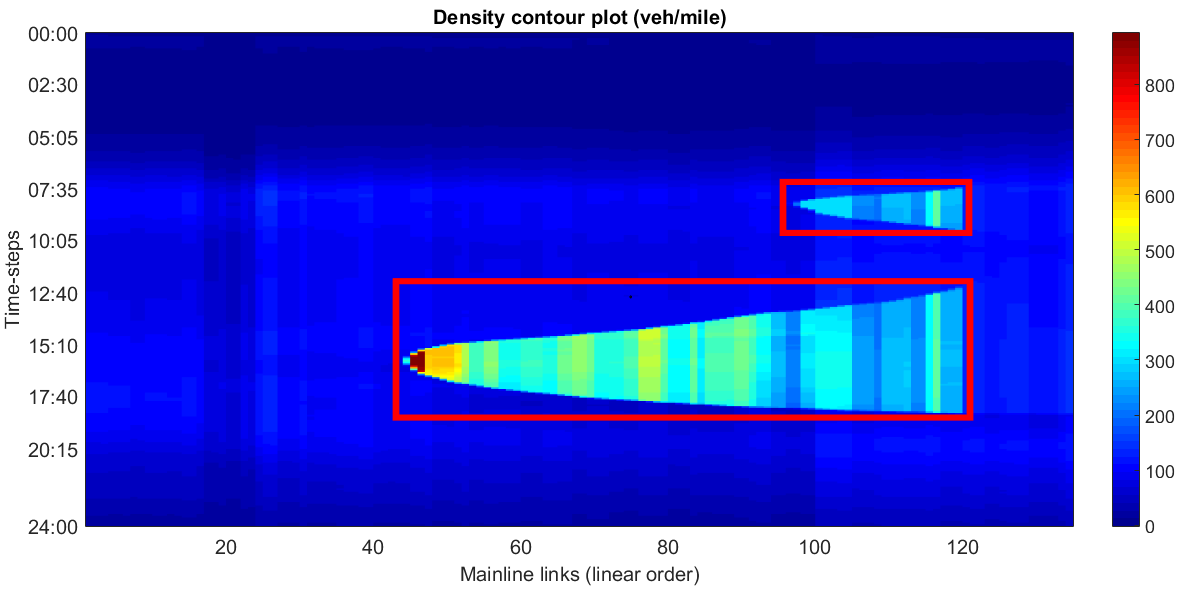
\includegraphics[width=4in]{figures/beats_contour.png}
\end{frame}



\begin{frame}
	\frametitle{Performance and error calculation}
	\framesubtitle{Congestion Pattern matching (CP)~~~~~~~~~~(2)}
		\begin{itemize}
			\item A congestion density threshold is defined for each mainline link.
			\item Error calculation: 
				\begin{equation*}
					E_{CP}(\vec{k})=\frac{\sum_{t\in{\tau}}\sum_{i\in{M}}\mathds{1}_{Wrong\ congestion\ state\ pixels}}{\sum_{t\in{\tau}}\sum_{i\in{M}}\mathds{1}_{Pixels\ supposed\ to\ be\ congested}}
				\end{equation*}
		\end{itemize}
\end{frame}



\begin{frame}
	\centering
	\frametitle{Performance and error calculation}
	\framesubtitle{Congestion Pattern matching (CP)~~~~~~~~~~(3)}
	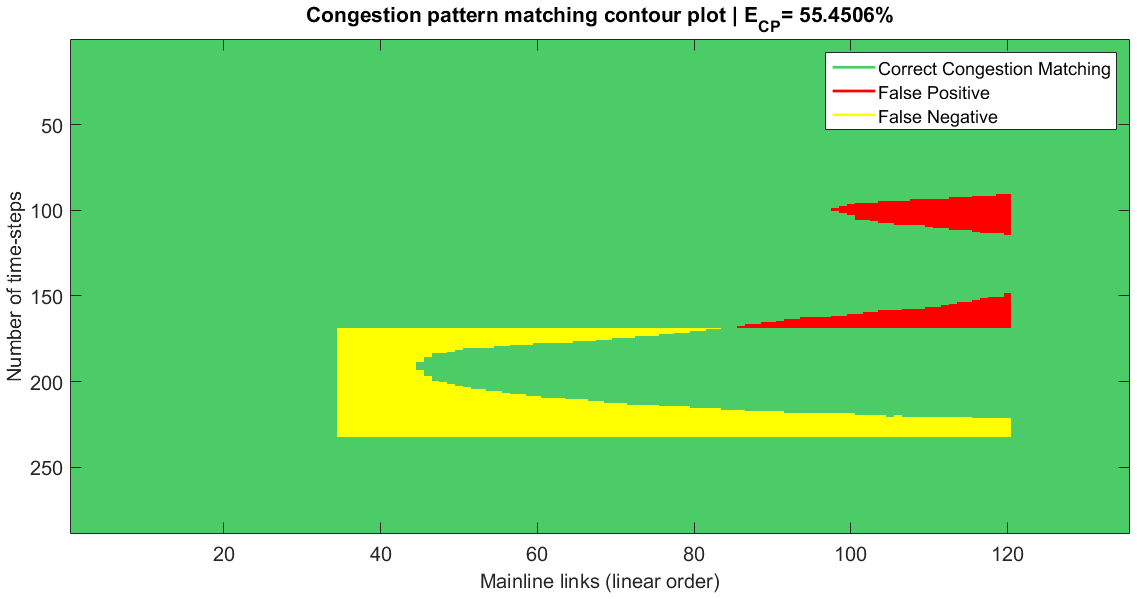
\includegraphics[width=4in]{figures/cp_example.png}
\end{frame}



\begin{frame}
	\frametitle{Problem Formulation}
	\framesubtitle{Fitness function}
	\begin{itemize}
		\item Components: 
		\begin{itemize}
			\item $\phi_{VHT}(\vec{k})=w_{1}.E_{VHT}(\vec{k}).\mathds{1}_{(E_{VHT}>U^{global})}$\\
			\item $\phi_{VMT}(\vec{k})=w_{2}.E_{VMT}(\vec{k}).\mathds{1}_{(E_{VMT}>U^{global})}$\\
			\item $\phi_{CP}(\vec{k})=w_{3}.E_{CP}(\vec{k}).\mathds{1}_{(E_{CP}>U^{global})}$\\	
		\end{itemize}
		~\\
		\item Objective function: 
		\begin{equation*}
			\Phi:
			\left|
	  		\begin{array}{rcl}
		    	\mathscr{B} & \longrightarrow &[0,100] \\
		    	\vec{k} & \longmapsto &  \phi_{VHT}(\vec{k})+\phi_{VMT}(\vec{k})+\phi_{CP}(\vec{k}) \\
		  	\end{array}
			\right.
		\end{equation*}
	\end{itemize}			
\end{frame}


\begin{frame}
	\frametitle{Problem Formulation}
	\framesubtitle{Optimization problem statement}
	\begin{align*}
	&minimize\ \ \ \ \Phi(\vec{k}) \\
	&s.t.\ \ \ \ 	\forall i\in \llbracket 1,\gamma \rrbracket,\ \Delta_{i}^{-}\leq |\sum\limits_{j\in g_{i}}\sigma_{j}.k_{j}.\Theta| \leq \Delta_{i}^{+} \nonumber\\
	&and\ \widetilde{VMT}^{-}\leq\mathlarger{\sum\limits_{i\in K}}\biggl[\sigma_{i}.k_{i}.\Theta.	\sum\limits_{\underset{j>i}{j\in T}}L_{j}\biggr]+VMT^{ref}\leq \widetilde{VMT}^{+}\nonumber \\	
	&and\ \vec{k} \in \mathscr{B} \nonumber
	\end{align*}
\end{frame}


\begin{frame}
	\frametitle{Numerical method}
	\framesubtitle{Requirements}
	\begin{itemize}
		\item Non-linear, non-convex black-box imputation problem in continuous domain
		\item Need for adaptive method
		\item Execution time does not matter
	\end{itemize}
\end{frame}


\begin{frame}
	\frametitle{Numerical method}
	\framesubtitle{Covariance Matrix Adaptation - Evolution Strategy (CMA-ES)}
	\begin{itemize}
		\item One of the most powerful evolutionary algorithms for single-objective real-valued optimization (very used) 
		\item "Designed for difficult non-linear non-convex black-box optimisation problems in continuous domain"
		\item "Typically applied to unconstrained or bounded constraint optimization problems, and search space dimensions between three and a hundred"
		\item Does not presume existence of approximate gradients : feasible on our non-smooth problem
		\item \em Adaptive \em algorithm : almost no parameter tuning $\rightarrow$ suitable to be used on several different freeways and days.
		\item Time does not matter for this initial study : not the fastest ES but good solution quality 	
	\end{itemize}
\end{frame}


\begin{frame}
	\frametitle{Numerical method}
	\framesubtitle{Linear constraints implementation: Single knob groups equations}
	$\forall\ i\in G\ s.t.\ Card(g_{i})=1,\ i.e.\ g_{i}=\{j\}\ :$
\begin{equation}
	\frac{\max{\big\{0;|\Delta_{i}^{-}|\big\}}}{\Theta}\leq k_{j} \leq \frac{\min{\big\{m_{j};|\Delta_{i}^{+}|\big\}}}{\Theta}
\end{equation}
\end{frame}


\begin{frame}
	\frametitle{Numerical method}
	\framesubtitle{Constraints implementation : multiple knob groups and $VMT^{a-priori}$ equations~~~~~~~~~(1)}
	\begin{itemize}
	 \item Linear constraints not implemented in CMA-ES source code $\Rightarrow$ project \& penalize.
	 \item Projection: \\ 
	 $minimize \ \ \ \ \ \ \norm{\vec{k}^{(p)}-\underline{\vec{k}}^{(p)}}_{2}$\\
$s.t.\ \ \ \forall i\in{G}, \ \ \Delta_{i}^{-}< |\sum_{j\in{g_{i}}} \sigma_{j}.k_{j}.\Theta|<\Delta_{i}^{+}$\\
$and\ \widetilde{VMT}^{-}\leq\mathlarger{\sum\limits_{i\in K}}\biggl[\sigma_{i}.k_{i}.\Theta.	\sum\limits_{\underset{j>i}{j\in T}}L_{j}\biggr]+VMT^{ref}\leq \widetilde{VMT}^{+}\nonumber $\\
$and\ \ \ \ \vec{k}^{(p)}\in \mathscr{B}$\\
	\end{itemize}\end{frame}


\begin{frame}
	\frametitle{Numerical method}
	\framesubtitle{Constraints implementation : multiple knob groups and $VMT^{a-priori}$ equations~~~~~~~~~(2)}
	\begin{figure}
		\centering
		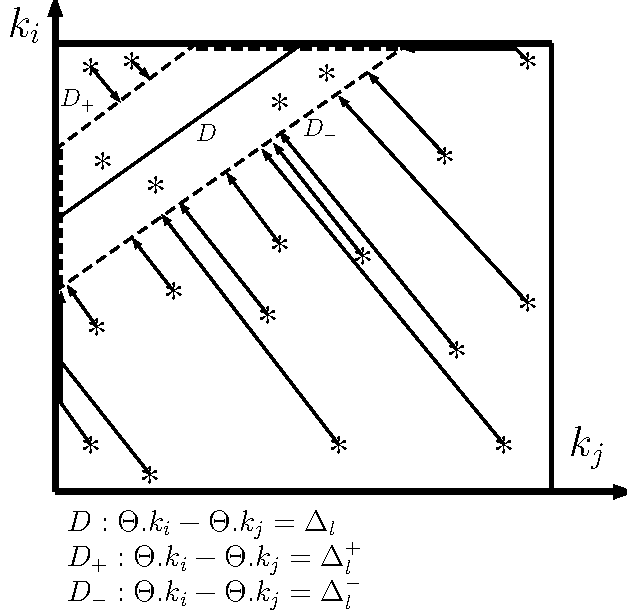
\includegraphics[width=2.5in]{figures/proj.pdf}	
	\end{figure}
\end{frame}


\begin{frame}
	\frametitle{Numerical method}
	\framesubtitle{Constraints implementation : multiple knob groups and $VMT^{a-priori}$ equations~~~~~~~~~(3)}
	\begin{itemize}
	 \item Penalization:
	 \begin{equation*}
	E_{proj}(\underline{\vec{k}}^{(p)},\vec{k}^{(p)})=\frac{\norm{\vec{k}^{(p)}-\underline{\vec{k}}^{(p)}}_{2}}{\norm{\begin{bmatrix}m_{1}\\m_{2}\\\vdots\\m_{\kappa}\end{bmatrix}-\begin{bmatrix}0\\0\\\vdots\\0\end{bmatrix}}_{2}}
	\end{equation*}
	\item The fitness function becomes: 
	\begin{equation*}
		J:
		\left|
  		\begin{array}{rcl}
    	\mathscr{B} & \longrightarrow &[0,100] \\
    	\underline{\vec{k}}^{(p)} & \longmapsto &  \Phi(\vec{k}^{(p)})+w_{4}.E_{proj}(\underline{\vec{k}}^{(p)},\vec{k}^{(p)}) \\
  	\end{array}
	\right.
	\end{equation*}
	\end{itemize}
\end{frame}


\begin{frame}
	\frametitle{Experiment settings}
	\framesubtitle{Data}
	\begin{itemize}
		\item Freeway 210 East in Los Angeles, average of 5 Tuesdays in fall 2104.
		\item  5-min measurements distributed as follows:
		\begin{itemize}
			\item 33/135 monitored mainline links
			\item 26/28 monitored on-ramps
			\item 15/25 monitored off-ramps
		\end{itemize}
		$\Rightarrow$ 12 knobs.
		\item Duration: 24 hours i.e.  289 time-steps (5min).
	\end{itemize}
\end{frame}

\begin{frame}
	\frametitle{Experiment settings}
	\framesubtitle{Model and simulator}
	\begin{itemize}
	\item Cell-transmission model\\
	~\\
	~\\
	\item Simulator: BeATS
	\end{itemize}
\end{frame}


\begin{frame}
	\frametitle{Experiment settings}
	\framesubtitle{Implementation of congestion pattern}
	\begin{figure}
		\centering
		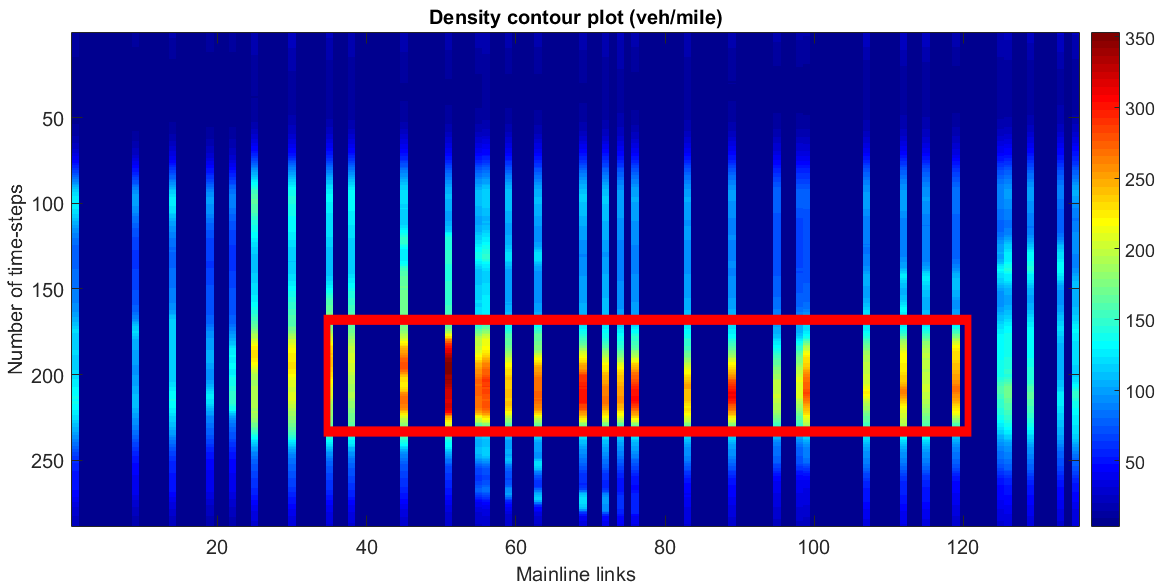
\includegraphics[width=4in]{figures/PeMS_contour.png}\\
		~\\
		$d_{i}^{*}=\frac{Link\ capacity}{Link\ free\ flow\ speed}+\delta$
	\end{figure}
\end{frame}


\begin{frame}
	\frametitle{Experiment results}
	\framesubtitle{General observations}
	\begin{itemize}
		\item Always converges\\
		~\\
		\item Limited result quality\\
		~\\
		\item No uniqueness\\
	\end{itemize}	
\end{frame}

\begin{frame}
	\frametitle{Experiment results}
	\framesubtitle{Overview}
	\begin{figure}
		\centering
		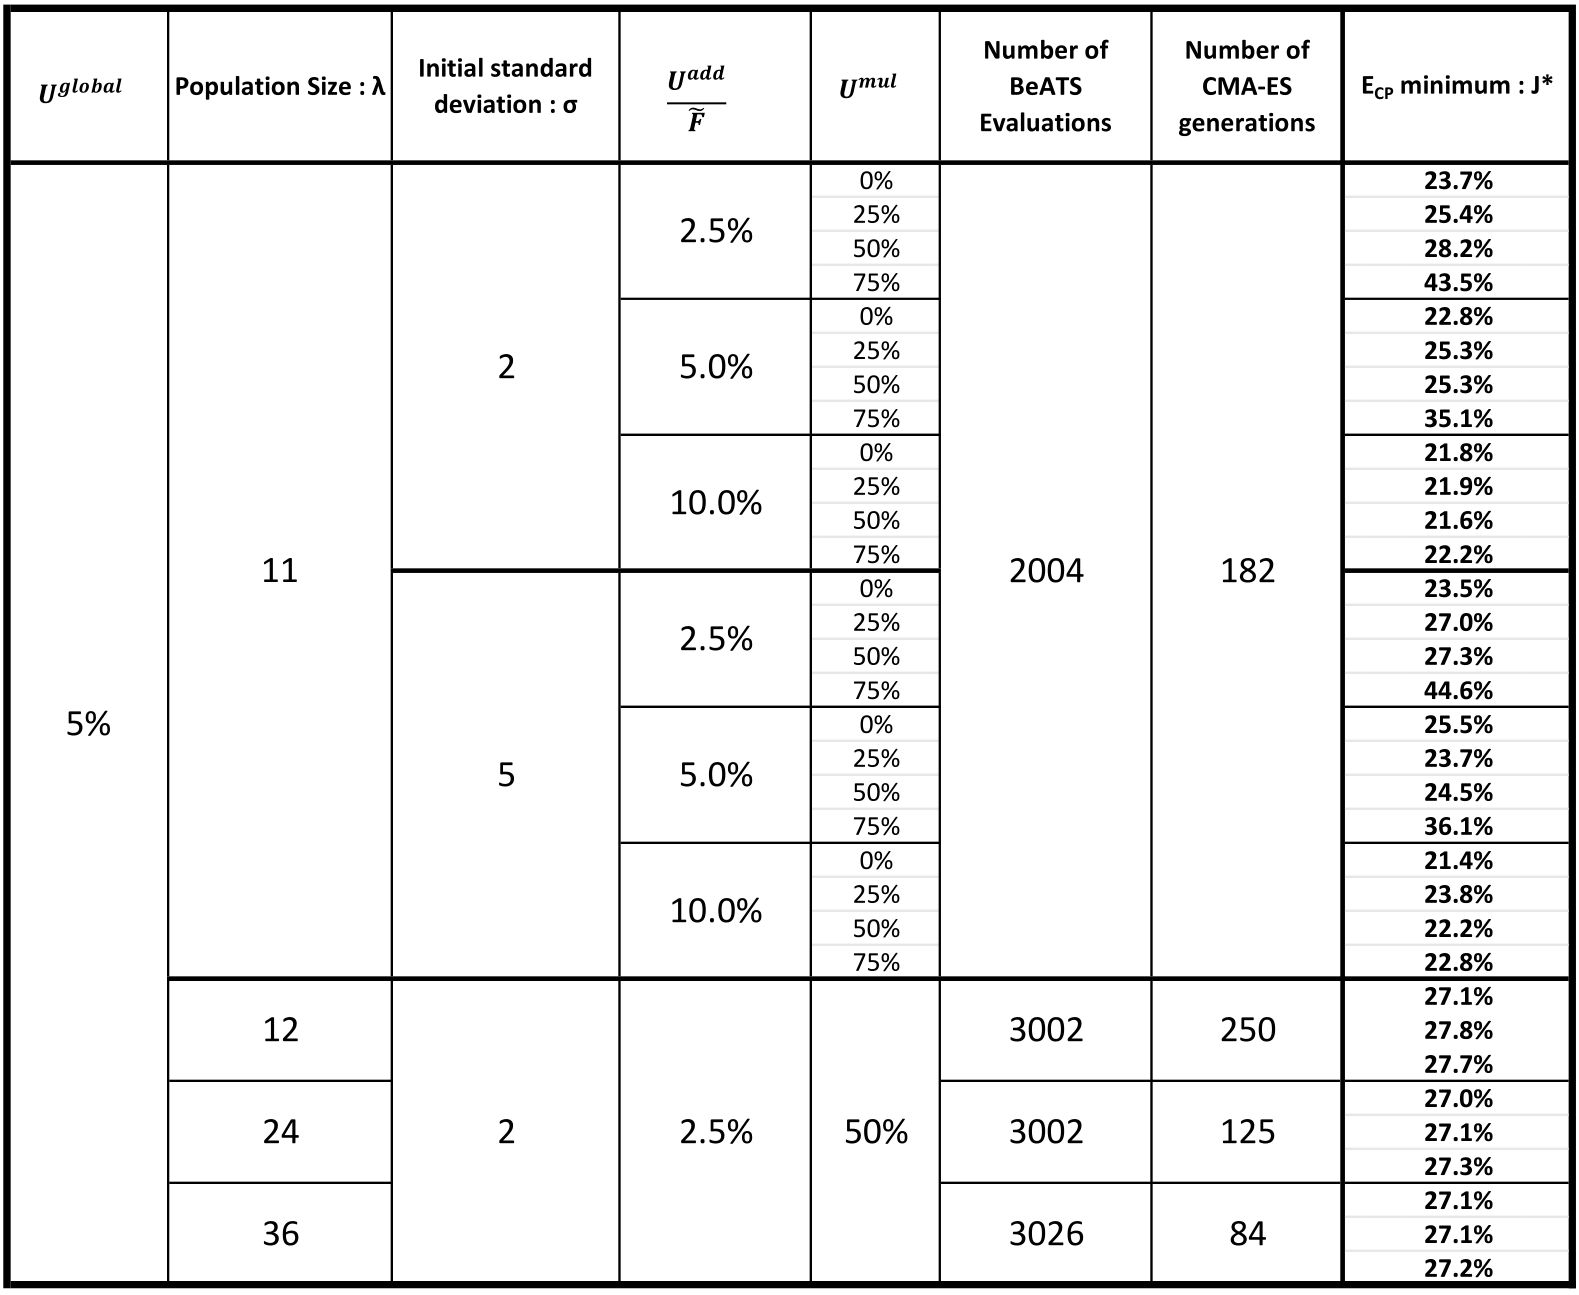
\includegraphics[width=3in]{figures/results_array.png}
	\end{figure}
\end{frame}
	
\begin{frame}
	\frametitle{Experiment results}
	\framesubtitle{Typical execution}
	\begin{figure}
		\centering
		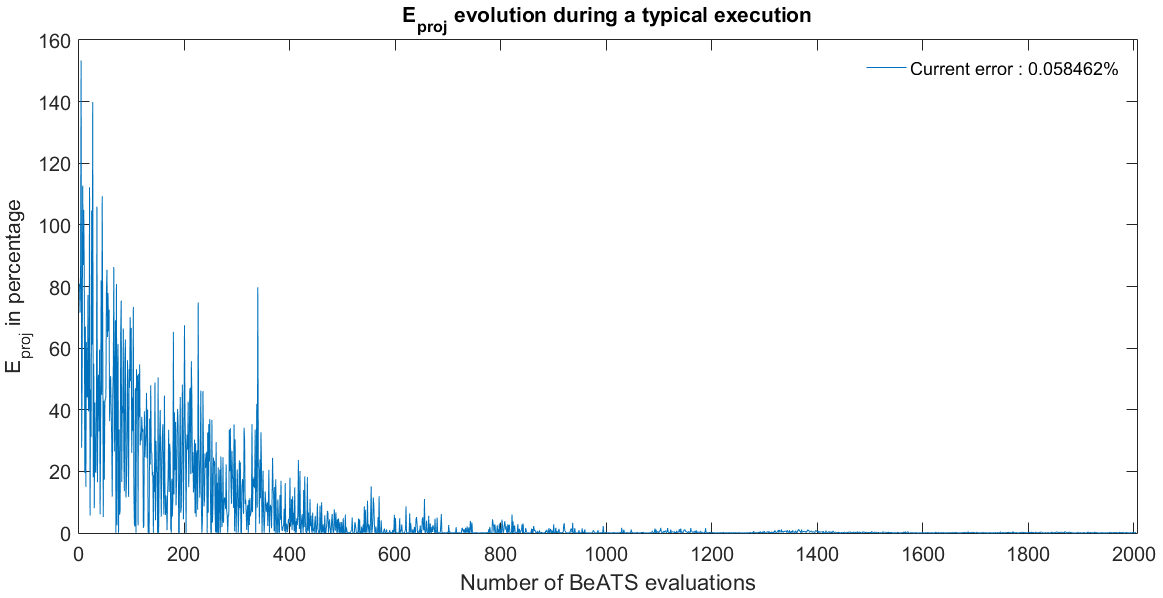
\includegraphics[width=4.5in]{figures/results_figures/eprojexample.png}
	\end{figure}
\end{frame}

\begin{frame}
	\frametitle{Experiment results}
	\framesubtitle{Typical execution}
	\begin{figure}
		\centering
		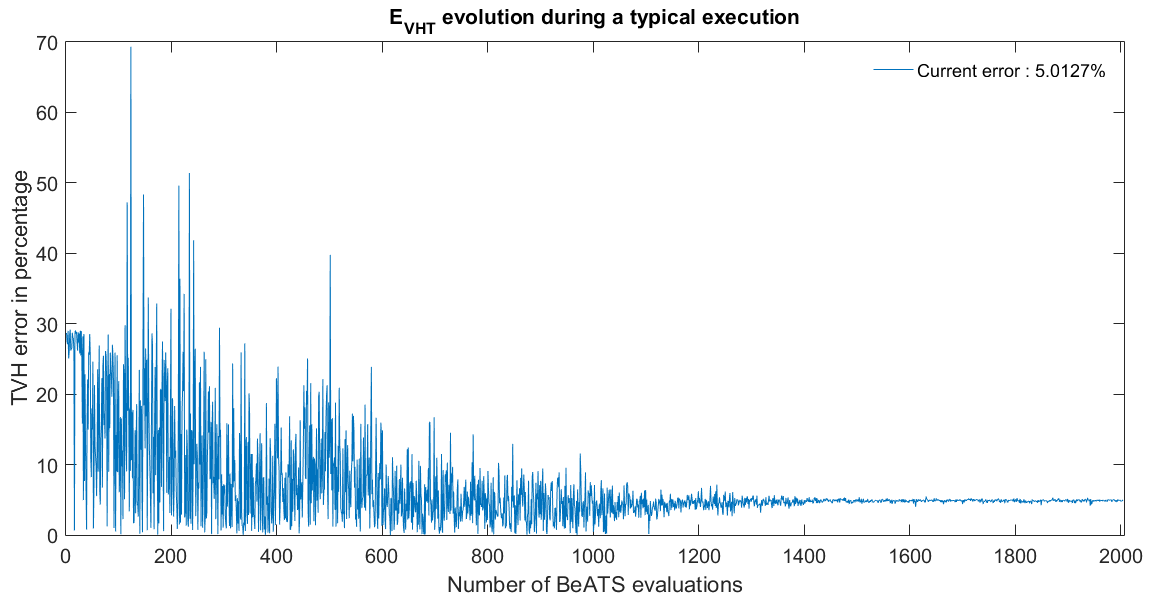
\includegraphics[width=4.5in]{figures/results_figures/VHTexample.png}
	\end{figure}
\end{frame}

\begin{frame}
	\frametitle{Experiment results}
	\framesubtitle{Typical execution}
	\begin{figure}
		\centering
		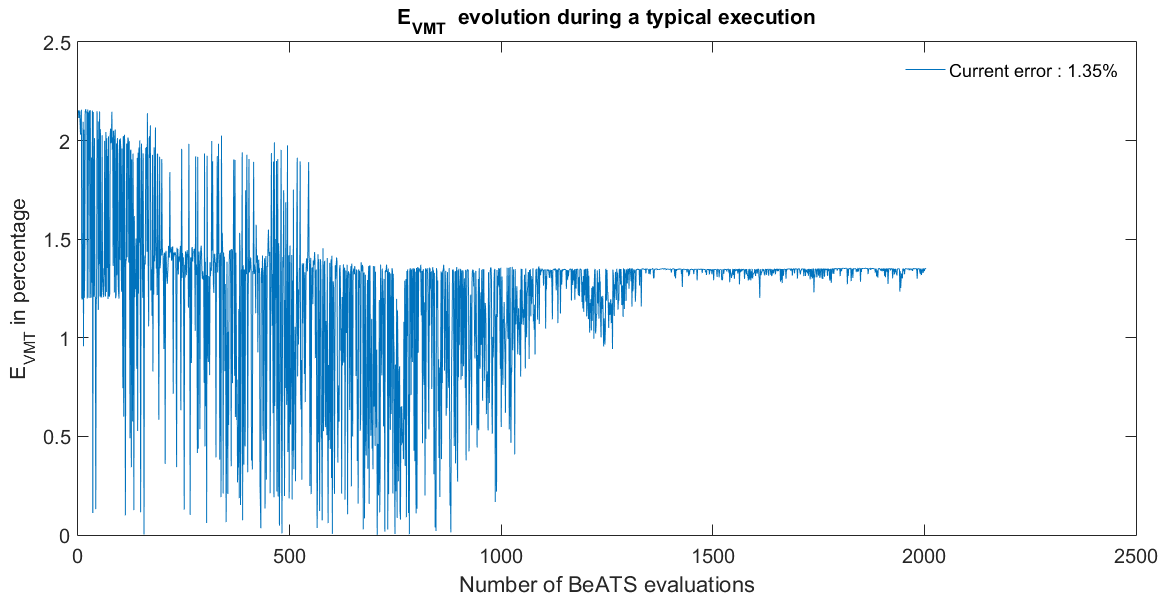
\includegraphics[width=4.5in]{figures/results_figures/VMTexample.png}
	\end{figure}
\end{frame}

\begin{frame}
	\frametitle{Experiment results}
	\framesubtitle{Typical execution}
	\begin{figure}
		\centering
		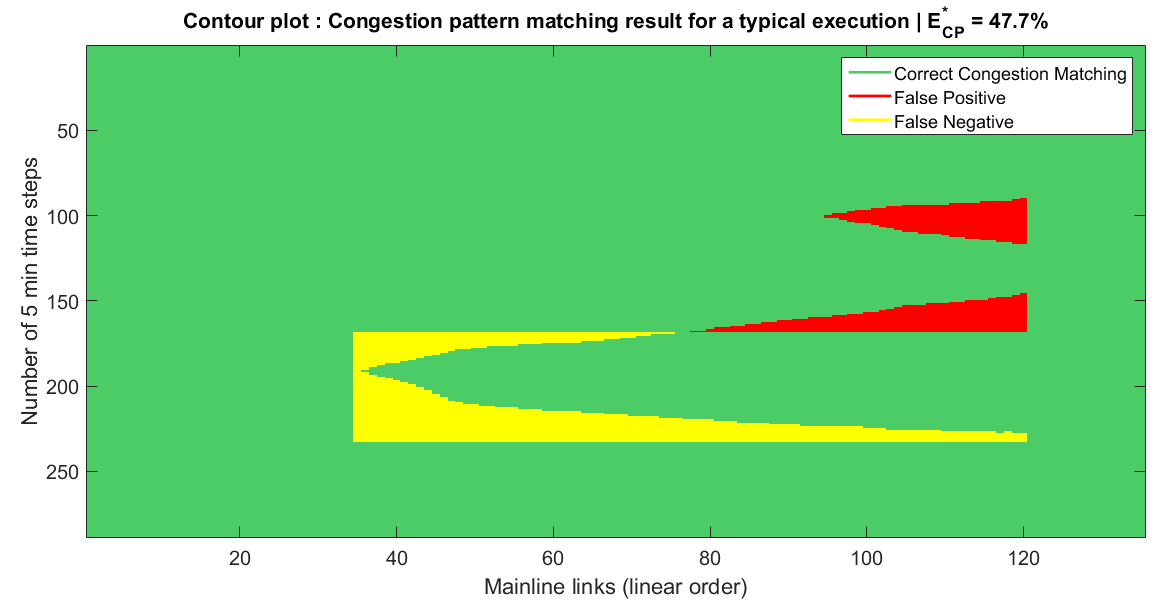
\includegraphics[width=4.5in]{figures/results_figures/typicalcpexample.png}
	\end{figure}
\end{frame}

\begin{frame}
	\frametitle{Experiment results}
	\framesubtitle{Typical execution}
	\begin{figure}
		\centering
		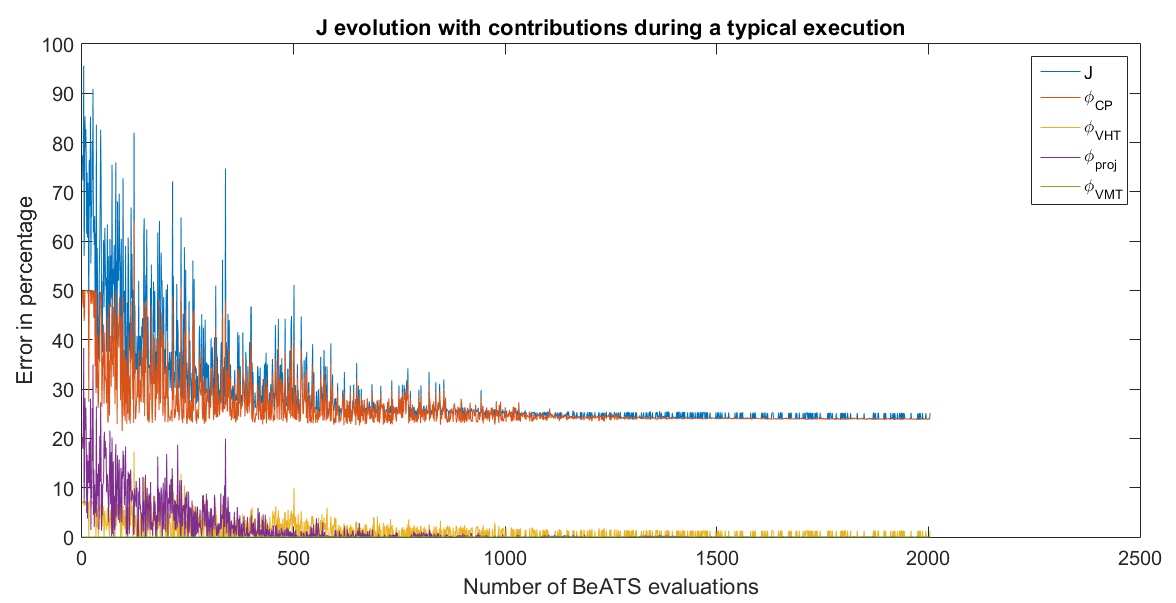
\includegraphics[width=4.5in]{figures/results_figures/contributionsexample.png}
	\end{figure}
\end{frame}

\begin{frame}
	\frametitle{Experiment results}
	\framesubtitle{Typical execution}
	\begin{figure}
		\centering
		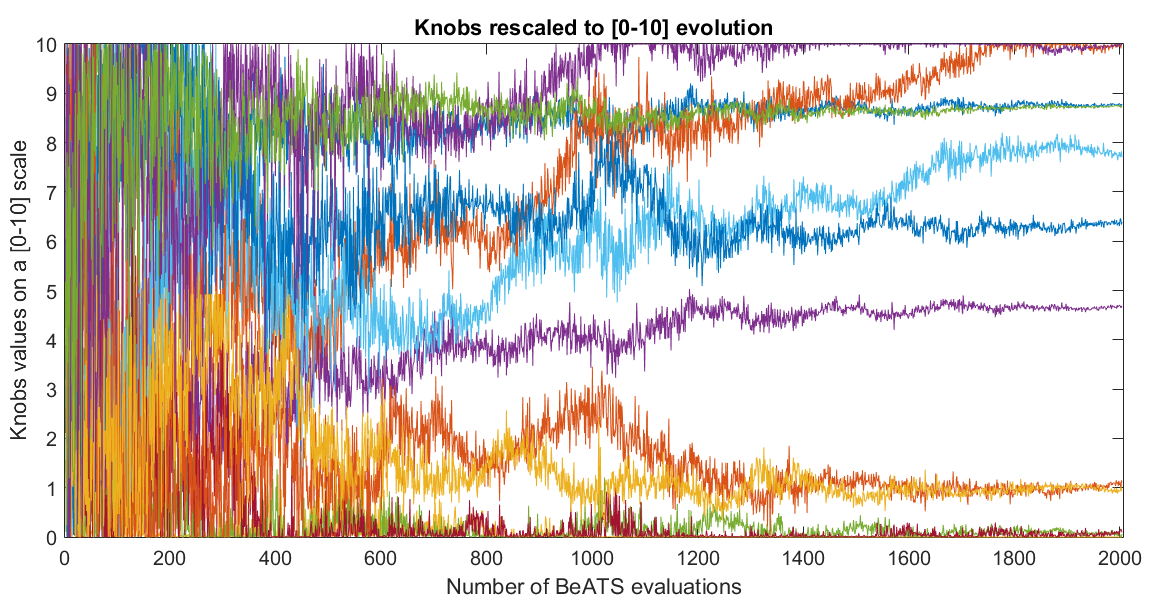
\includegraphics[width=4.5in]{figures/results_figures/typicalknobs.png}
	\end{figure}
\end{frame}

\begin{frame}
	\frametitle{Experiment results}
	\framesubtitle{Typical execution}
	\begin{figure}
		\centering
		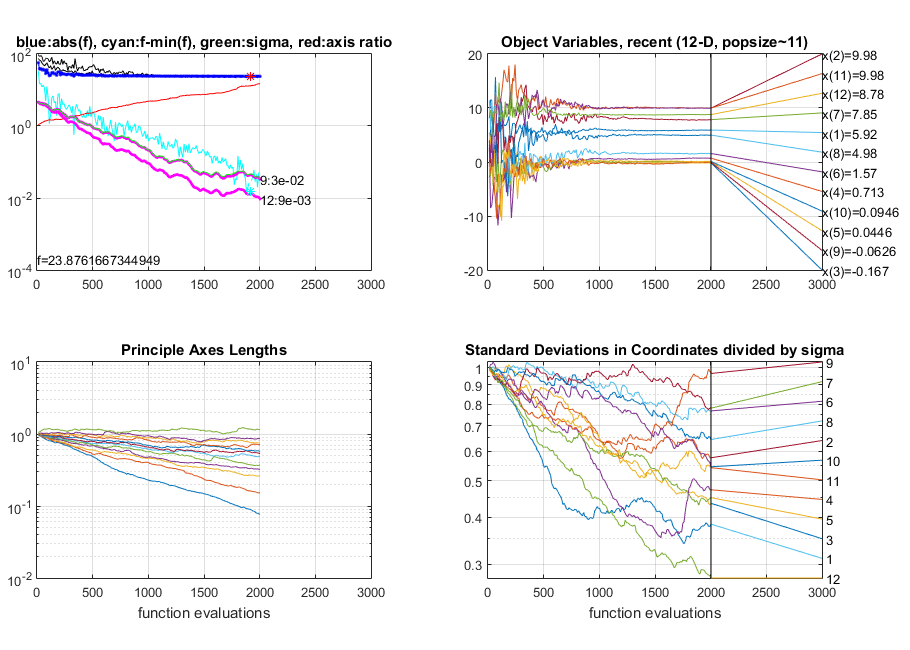
\includegraphics[width=4.5in]{figures/results_figures/cmaesexample.png}
	\end{figure}
\end{frame}



\begin{frame}
	\frametitle{Experiment results}
	\framesubtitle{Effect of $U^{mul}$}
	\begin{figure}
		\centering
		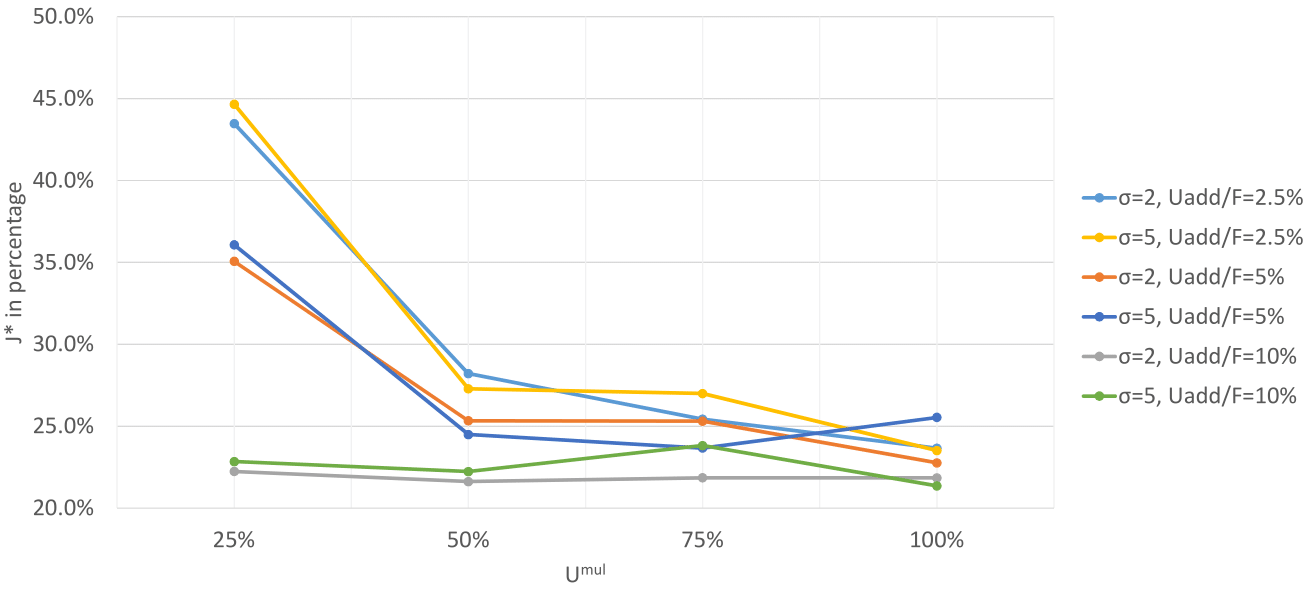
\includegraphics[width=4.5in]{figures/umul.png}
	\end{figure}
\end{frame}

\begin{frame}
	\frametitle{Experiment results}
	\framesubtitle{$U^{mul}=25\% $}
	\begin{figure}
		\centering
		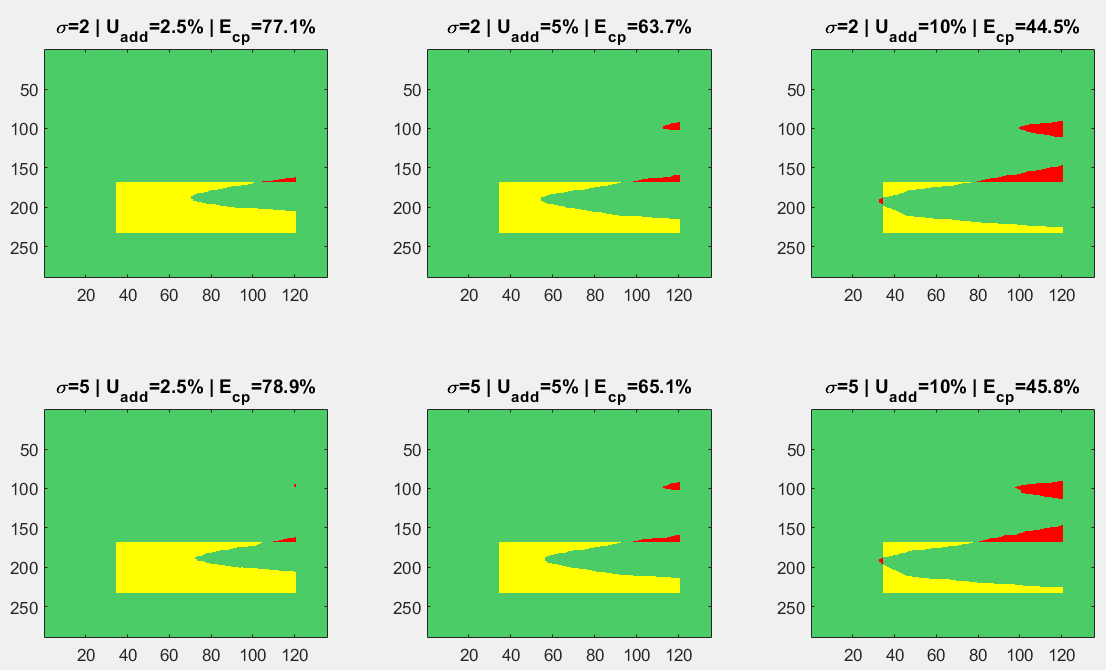
\includegraphics[width=4.5in]{figures/results_figures/Umul/cp_Umul_25_lambda_11.png}
	\end{figure}
\end{frame}

\begin{frame}
	\frametitle{Experiment results}
	\framesubtitle{$U^{mul}=25\% $}
	\begin{figure}
		\centering
		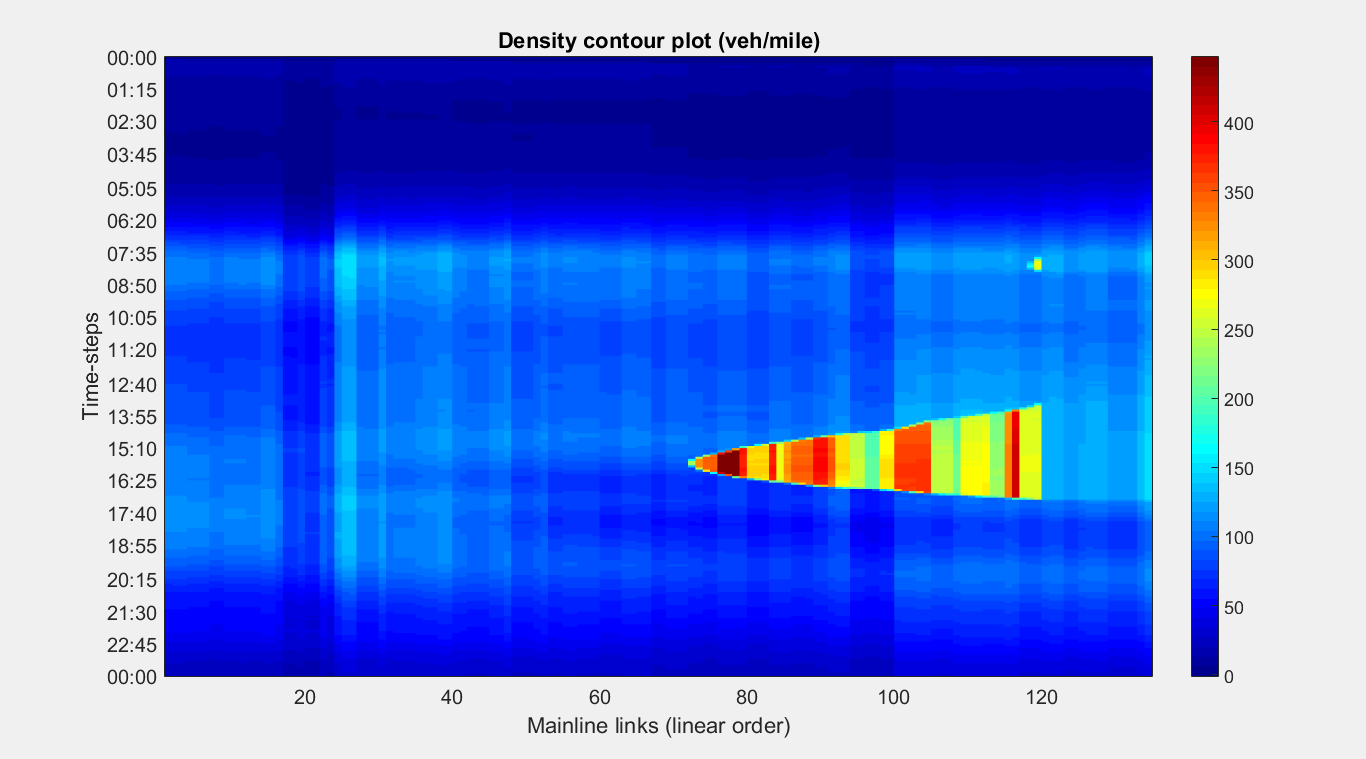
\includegraphics[width=4.5in]{figures/results_figures/Umul/13_2_too_tight_contour.png}
	\end{figure}
\end{frame}


\begin{frame}
	\frametitle{Experiment results}
	\framesubtitle{$U^{mul}=25\% $}
	\begin{figure}
		\centering
		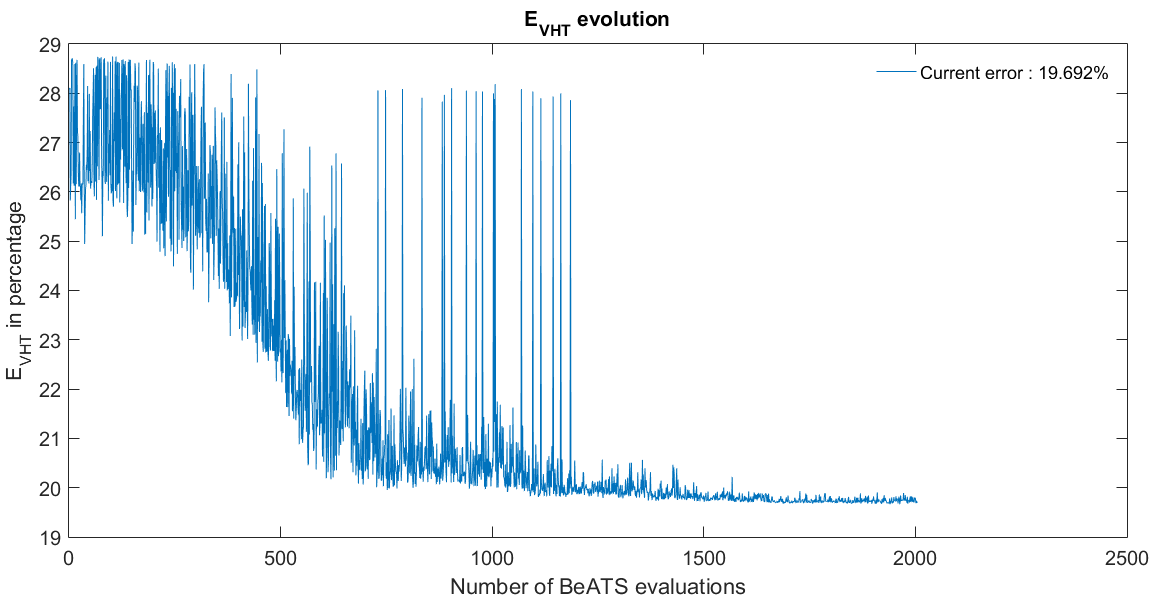
\includegraphics[width=4.5in]{figures/results_figures/Umul/bad_vht.png}
	\end{figure}
\end{frame}

\begin{frame}
	\frametitle{Experiment results}
	\framesubtitle{$U^{mul}=50\% $}
	\begin{figure}
		\centering
		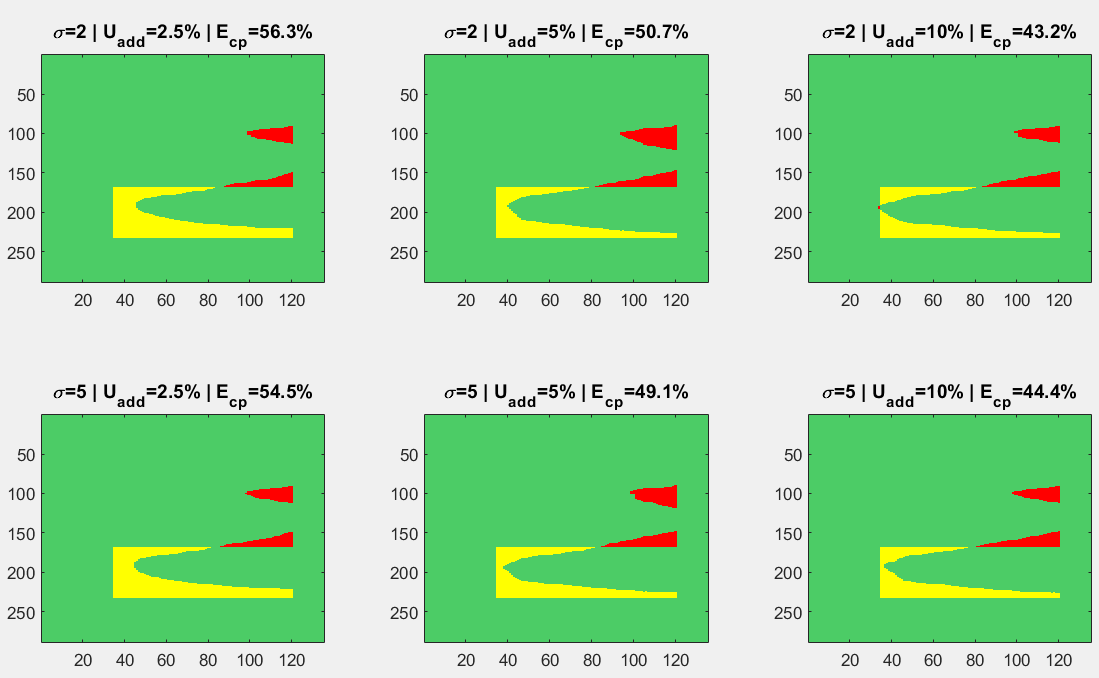
\includegraphics[width=4.5in]{figures/results_figures/Umul/cp_Umul_50_lambda_11.png}
	\end{figure}
\end{frame}

\begin{frame}
	\frametitle{$U^{mul}=75\% $}
	\framesubtitle{Effect of $U^{mul}$}
	\begin{figure}
		\centering
		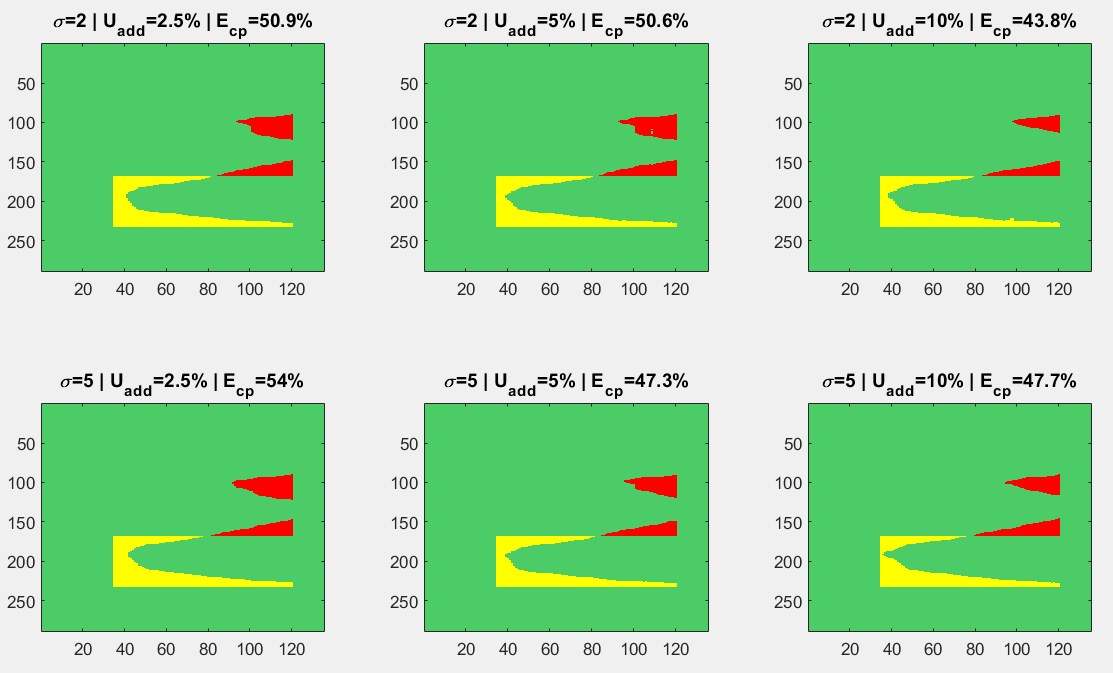
\includegraphics[width=4.5in]{figures/results_figures/Umul/cp_Umul_75_lambda_11.png}
	\end{figure}
\end{frame}

\begin{frame}
	\frametitle{$U^{mul}=100\% $}
	\framesubtitle{Effect of $U^{mul}$}
	\begin{figure}
		\centering
		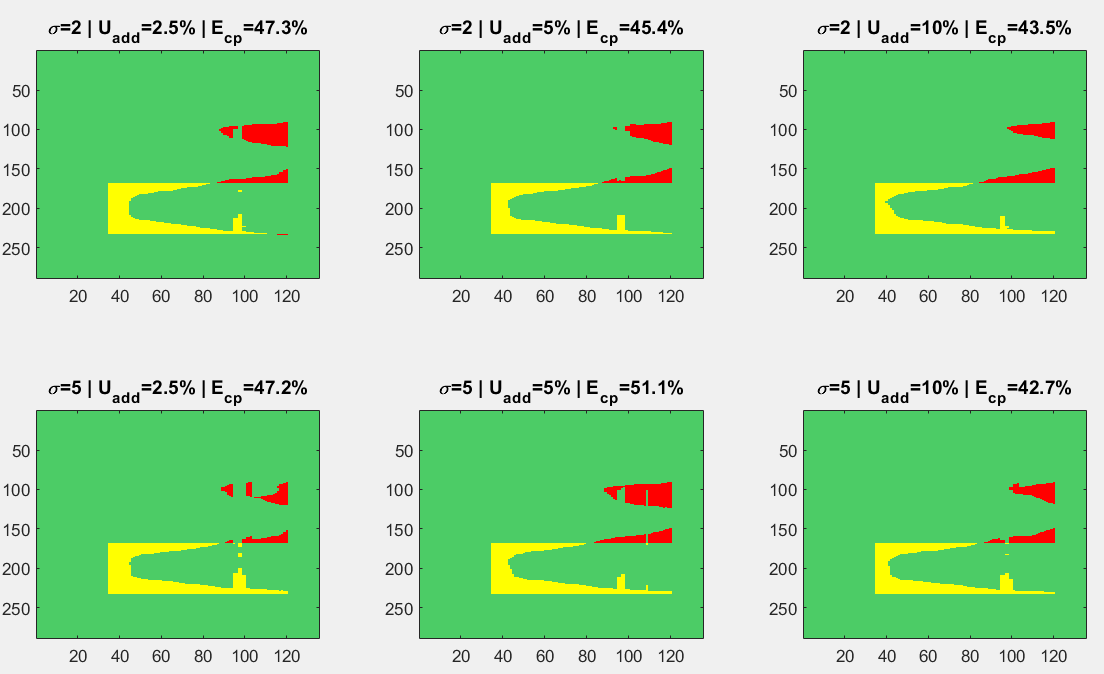
\includegraphics[width=4.5in]{figures/results_figures/Umul/cp_Umul_100_lambda_11.png}
	\end{figure}
\end{frame}


\begin{frame}
	\frametitle{$U^{mul}=25\% $}
	\framesubtitle{Effect of $U^{mul}$}
	\begin{figure}
		\centering
		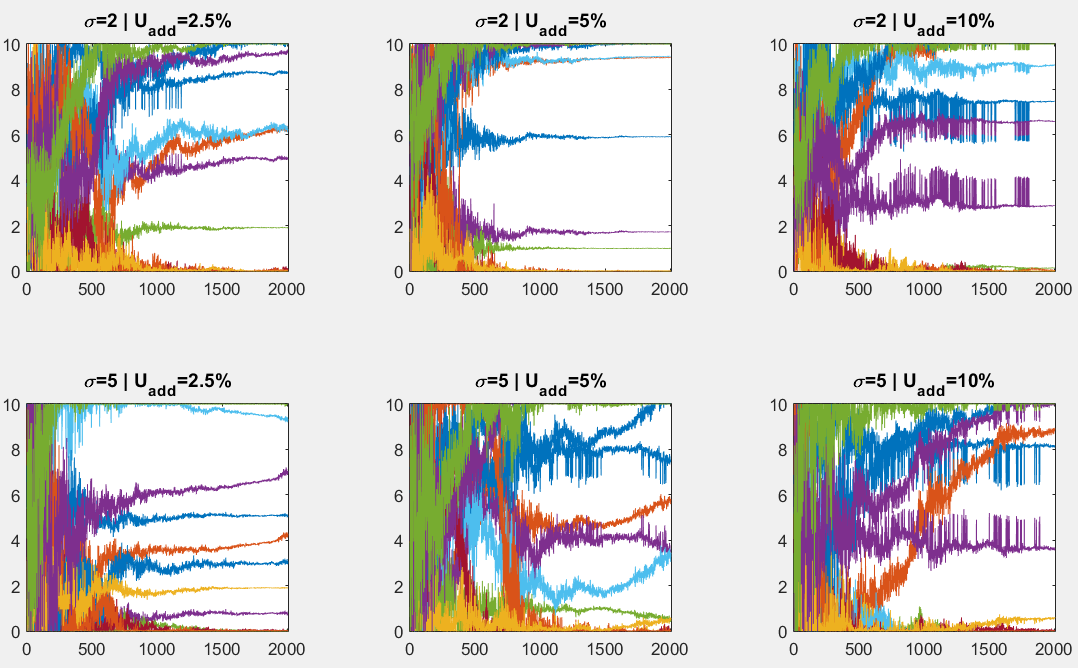
\includegraphics[width=4.5in]{figures/results_figures/Umul/knobs_Umul_25_lambda_11.png}
	\end{figure}
\end{frame}

\begin{frame}
	\frametitle{$U^{mul}=25\%$}
	\framesubtitle{Effect of $U^{mul}$}
	\begin{figure}
		\centering
		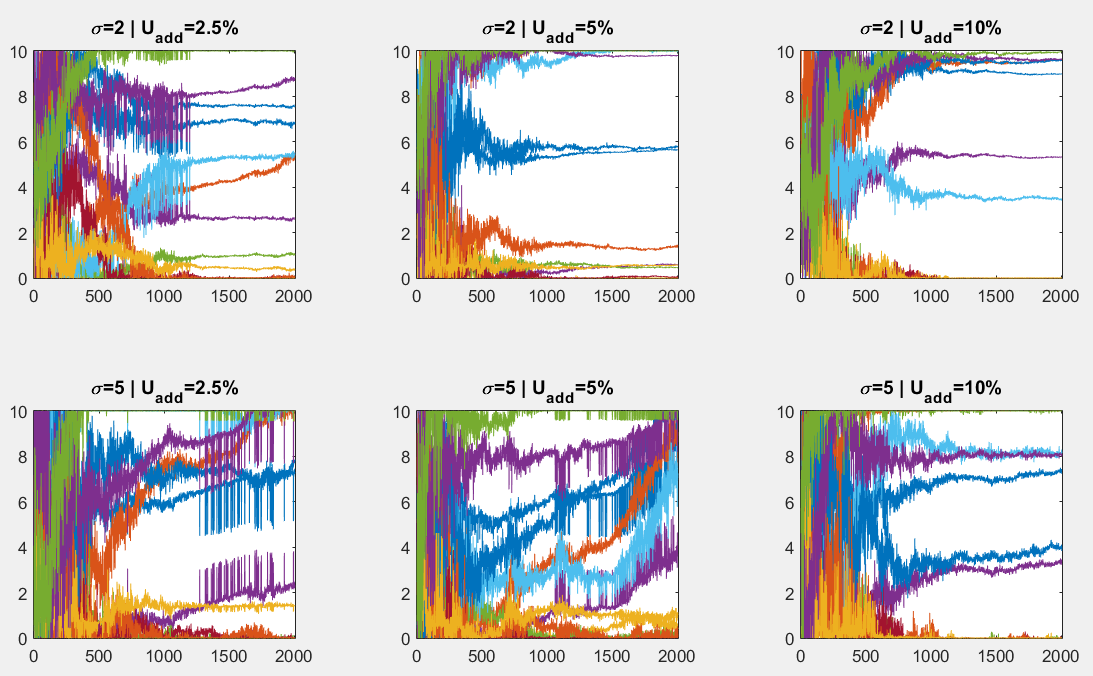
\includegraphics[width=4.5in]{figures/results_figures/Umul/knobs_Umul_50_lambda_11.png}
	\end{figure}
\end{frame}

\begin{frame}
	\frametitle{$U^{mul}=25\%$}
	\framesubtitle{Effect of $U^{mul}$}
	\begin{figure}
		\centering
		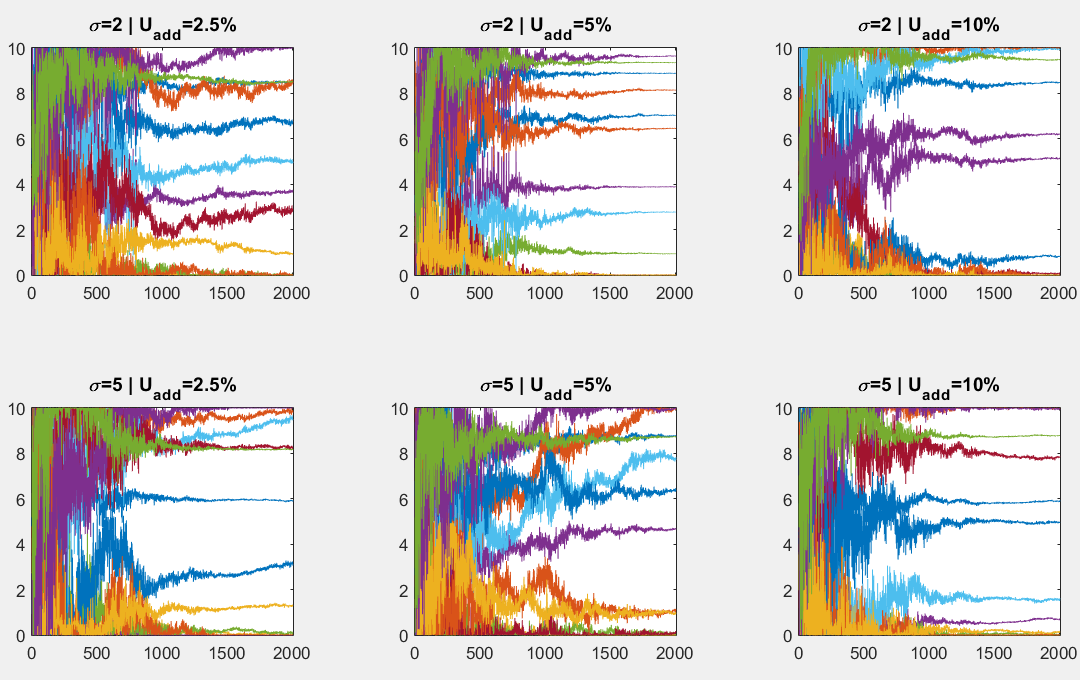
\includegraphics[width=4.5in]{figures/results_figures/Umul/knobs_Umul_75_lambda_11.png}
	\end{figure}
\end{frame}

\begin{frame}
	\frametitle{Experiment results}
	\framesubtitle{Effect of $U^{mul}$}
	\begin{figure}
		\centering
		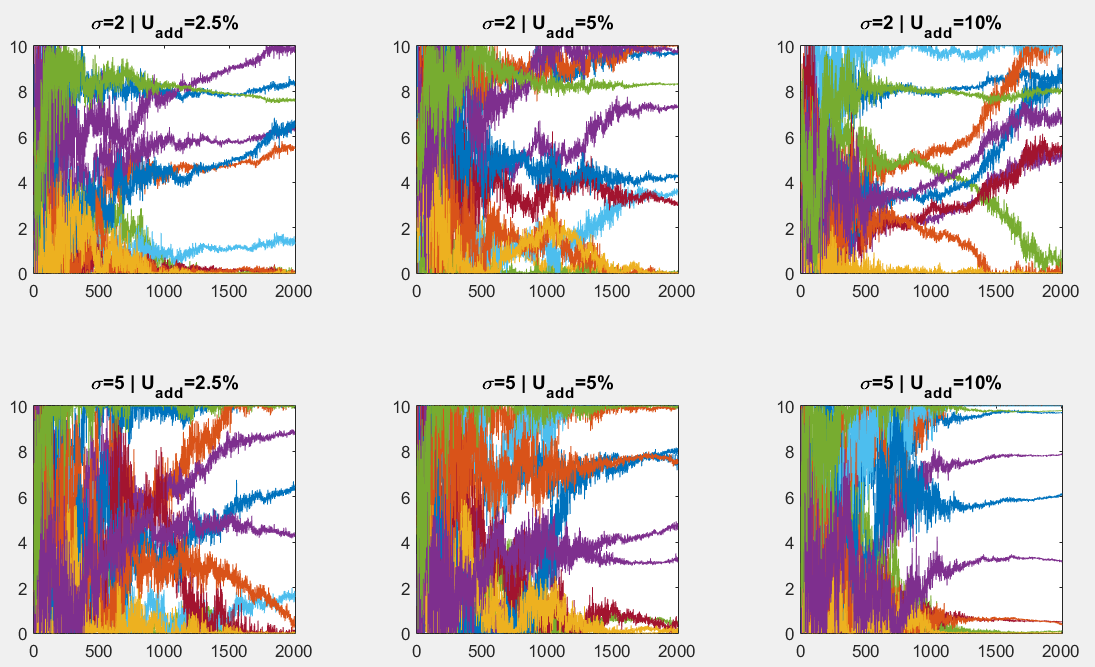
\includegraphics[width=4.5in]{figures/results_figures/Umul/knobs_Umul_100_lambda_11.png}
	\end{figure}
\end{frame}


\begin{frame}
	\frametitle{Experiment results}
	\framesubtitle{Effect of $U^{add}$}
	\begin{figure}
		\centering
		\includegraphics[width=4.5in]{figures/Uadd.png}
	\end{figure}
\end{frame}

\begin{frame}
	\frametitle{Experiment results}
	\framesubtitle{Effect of $U^{add}$}
	\begin{figure}
		\centering
		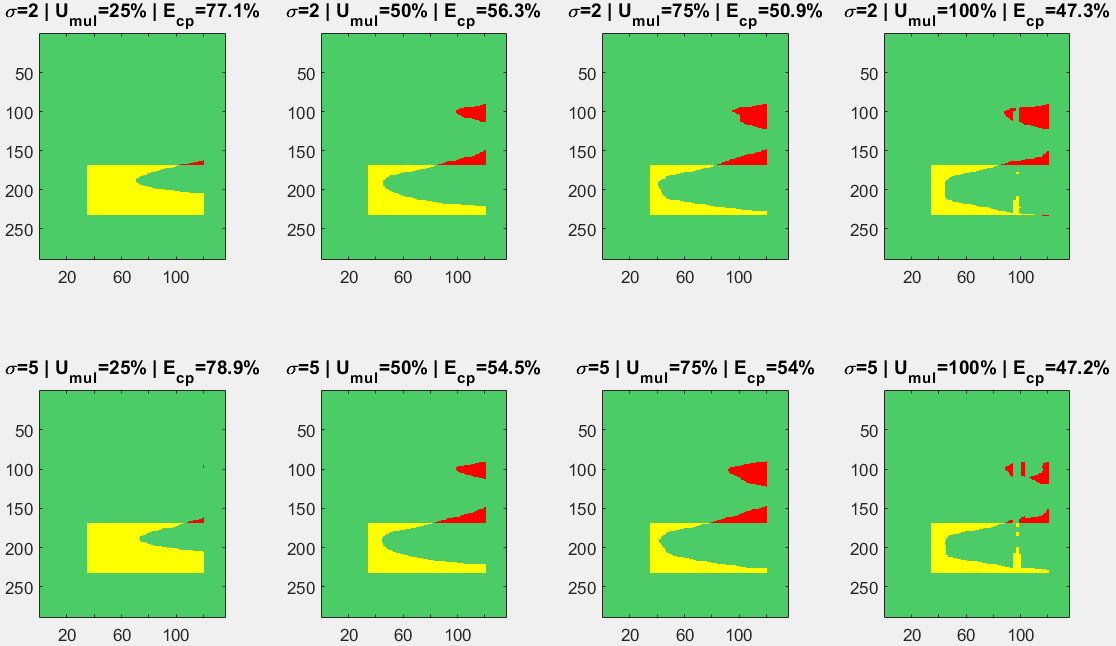
\includegraphics[width=4.5in]{figures/results_figures/Uadd/cp_Uadd_25_lambda_11.png}
	\end{figure}
\end{frame}

\begin{frame}
	\frametitle{Experiment results}
	\framesubtitle{Effect of $U^{add}$}
	\begin{figure}
		\centering
		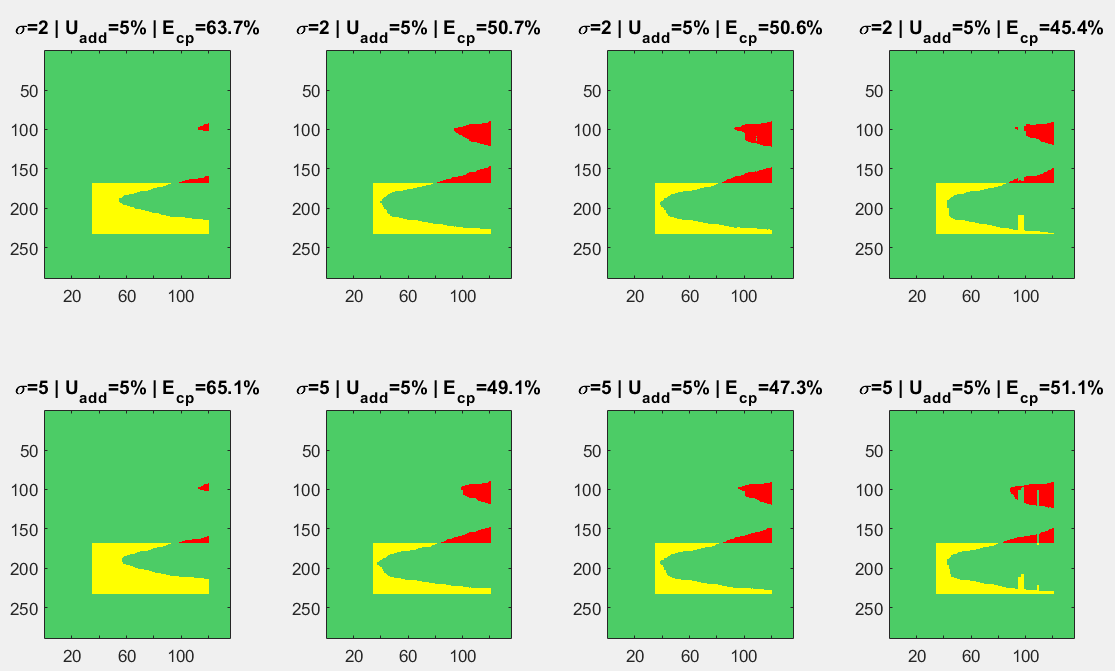
\includegraphics[width=4.5in]{figures/results_figures/Uadd/cp_Uadd_5_lambda_11.png}
	\end{figure}
\end{frame}

\begin{frame}
	\frametitle{Experiment results}
	\framesubtitle{Effect of $U^{add}$}
	\begin{figure}
		\centering
		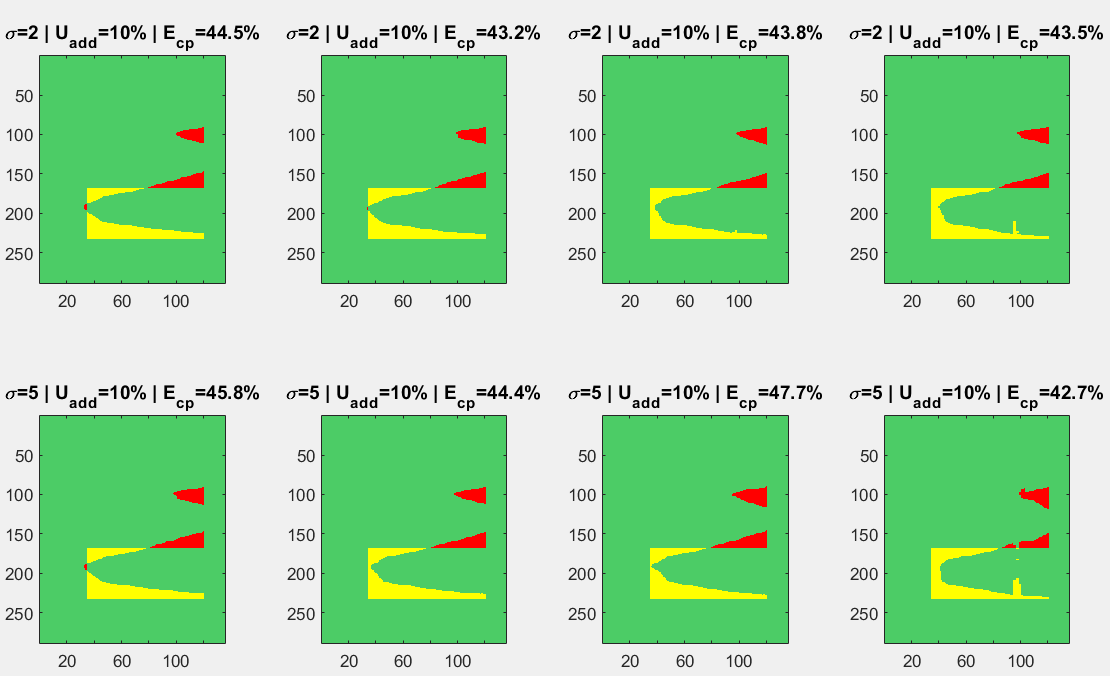
\includegraphics[width=4.5in]{figures/results_figures/Uadd/cp_Uadd_10_lambda_11.png}
	\end{figure}
\end{frame}

\begin{frame}
	\frametitle{Experiment results}
	\framesubtitle{Effect of $U^{add}$}
	\begin{figure}
		\centering
		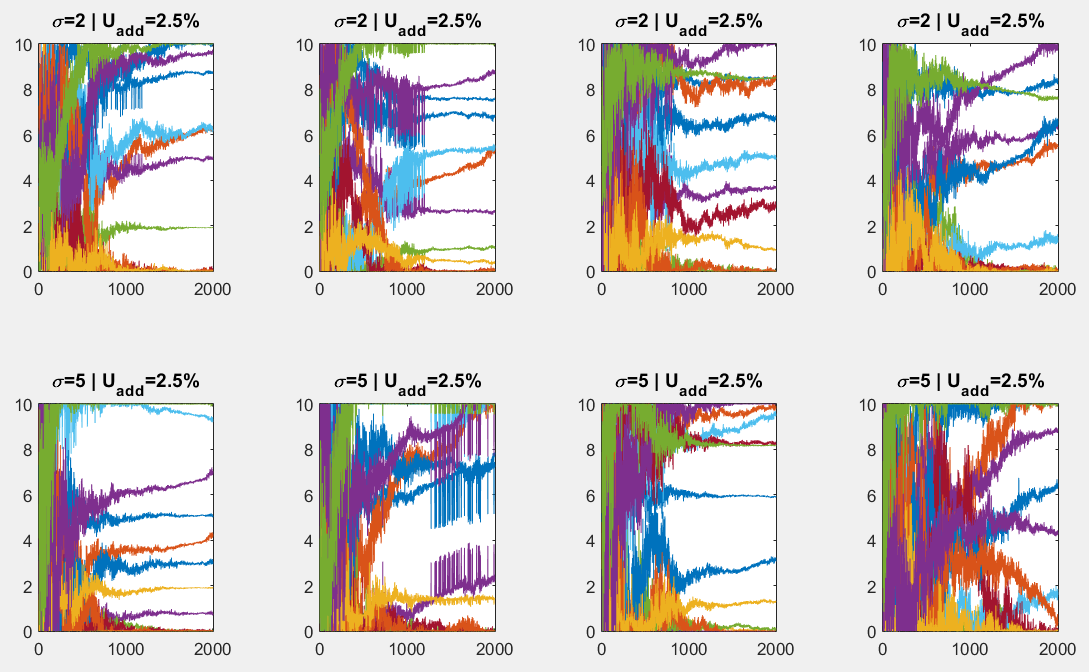
\includegraphics[width=4.5in]{figures/results_figures/Uadd/knobs_Uadd_25_lambda_11.png}
	\end{figure}
\end{frame}

\begin{frame}
	\frametitle{Experiment results}
	\framesubtitle{Effect of $U^{add}$}
	\begin{figure}
		\centering
		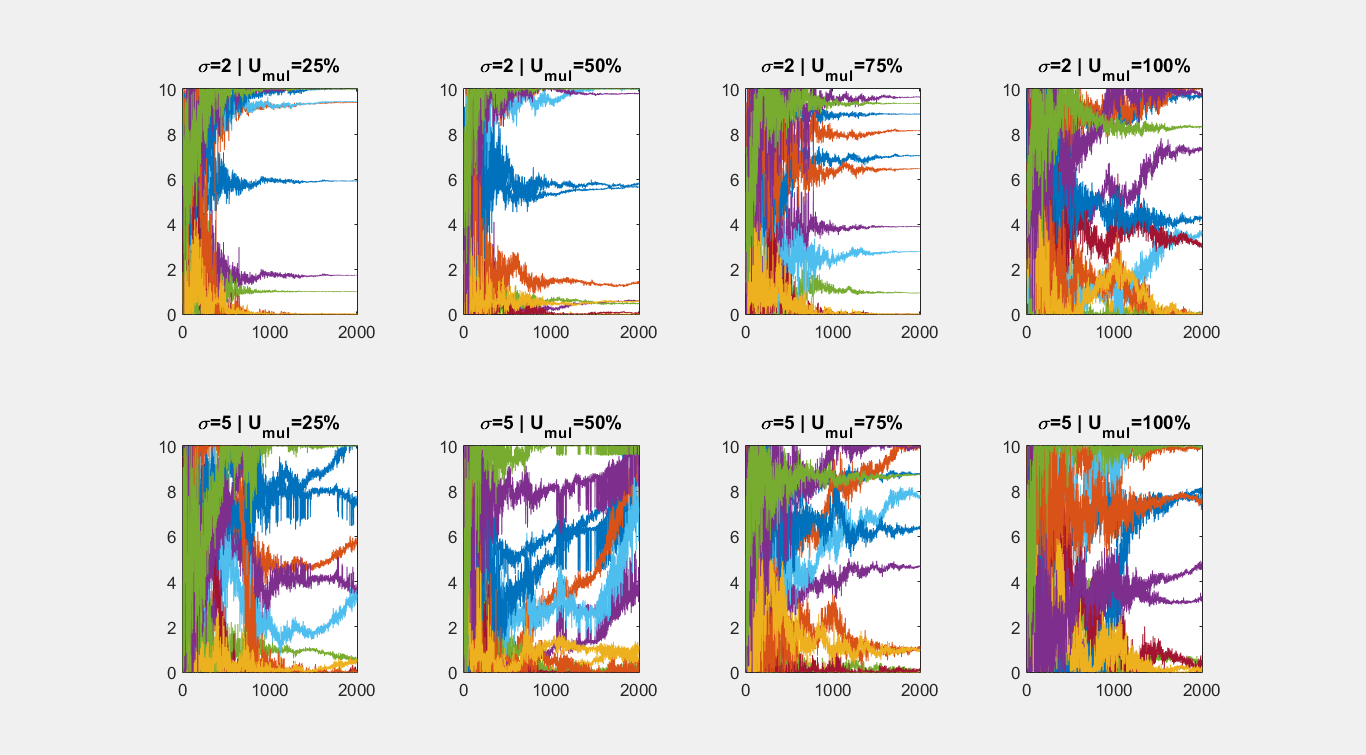
\includegraphics[width=4.5in]{figures/results_figures/Uadd/knobs_Uadd_5_lambda_11.png}
	\end{figure}
\end{frame}

\begin{frame}
	\frametitle{Experiment results}
	\framesubtitle{Effect of $U^{add}$}
	\begin{figure}
		\centering
		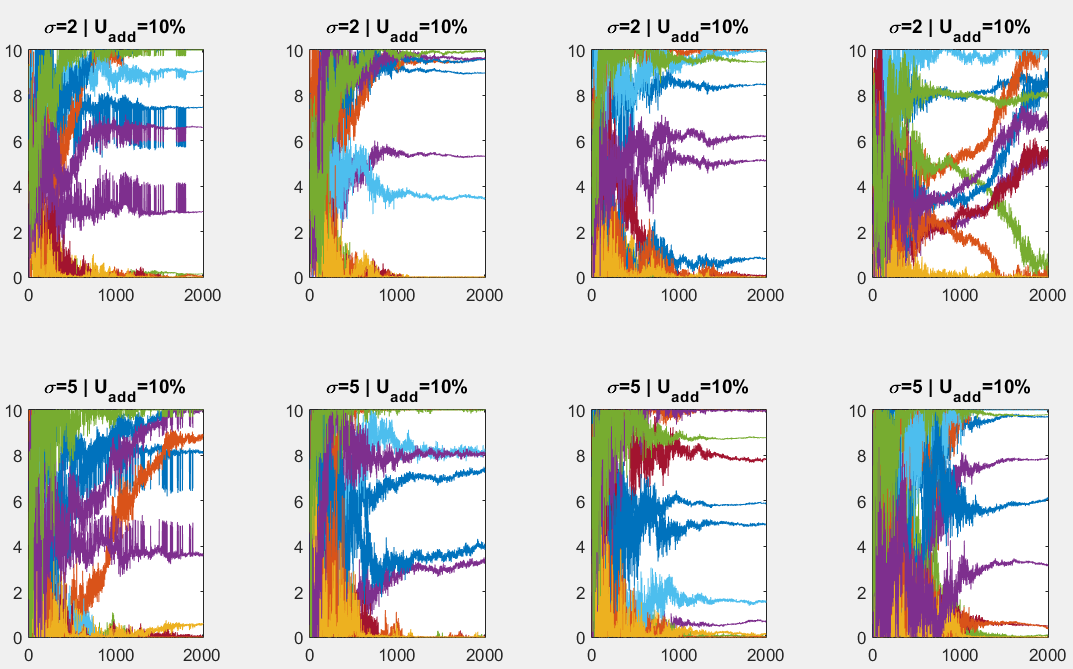
\includegraphics[width=4.5in]{figures/results_figures/Uadd/knobs_Uadd_10_lambda_11.png}
	\end{figure}
\end{frame}

\begin{frame}
	\frametitle{Experiment results}
	\framesubtitle{Effects of $\sigma$}
	\begin{figure}
		\centering
		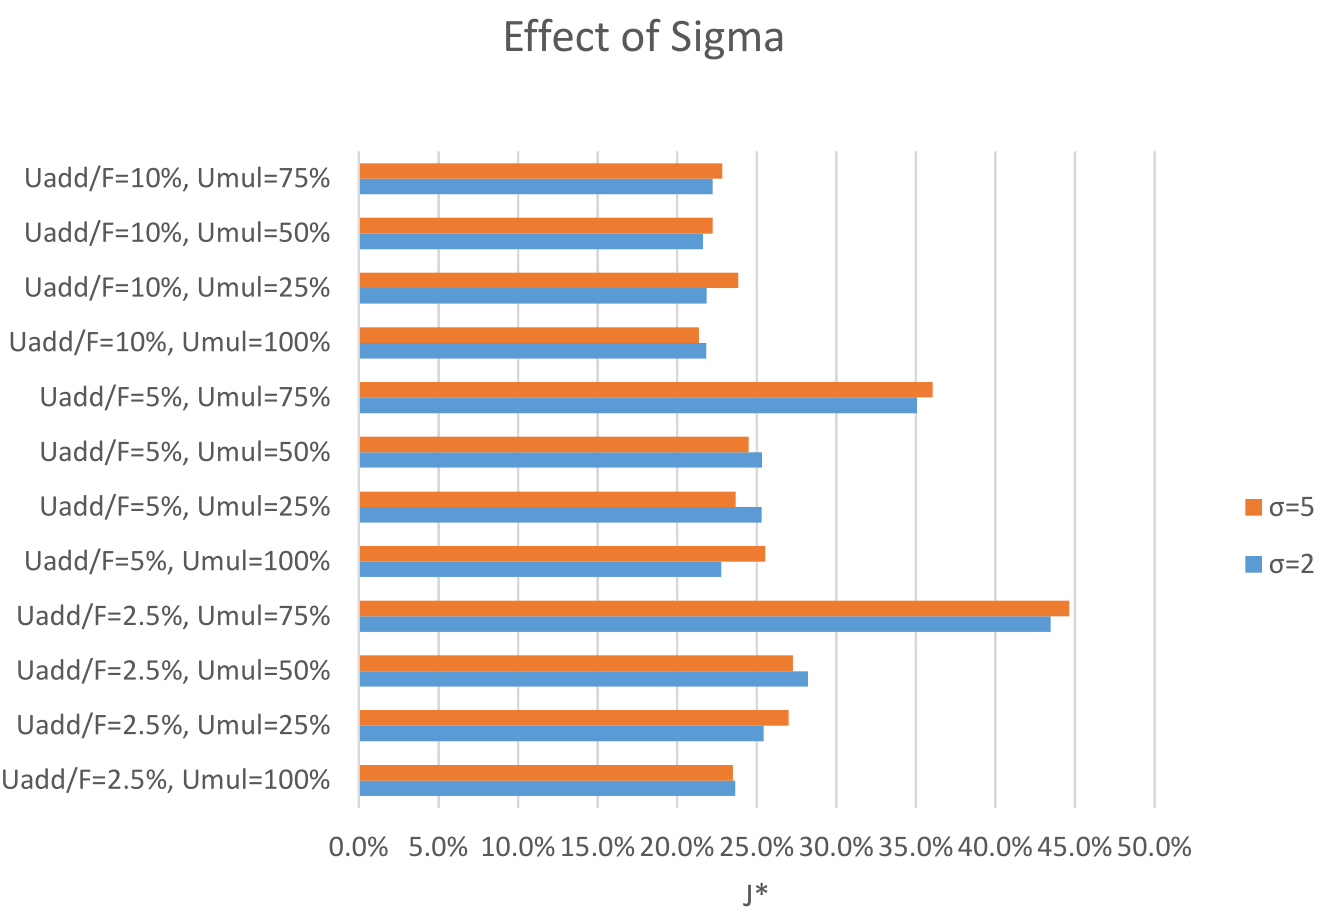
\includegraphics[width=4in]{figures/sigma.png}
	\end{figure}
\end{frame}


\begin{frame}
	\frametitle{Experiment results}
	\framesubtitle{Effects of $\lambda$}
	\begin{figure}
		\centering
		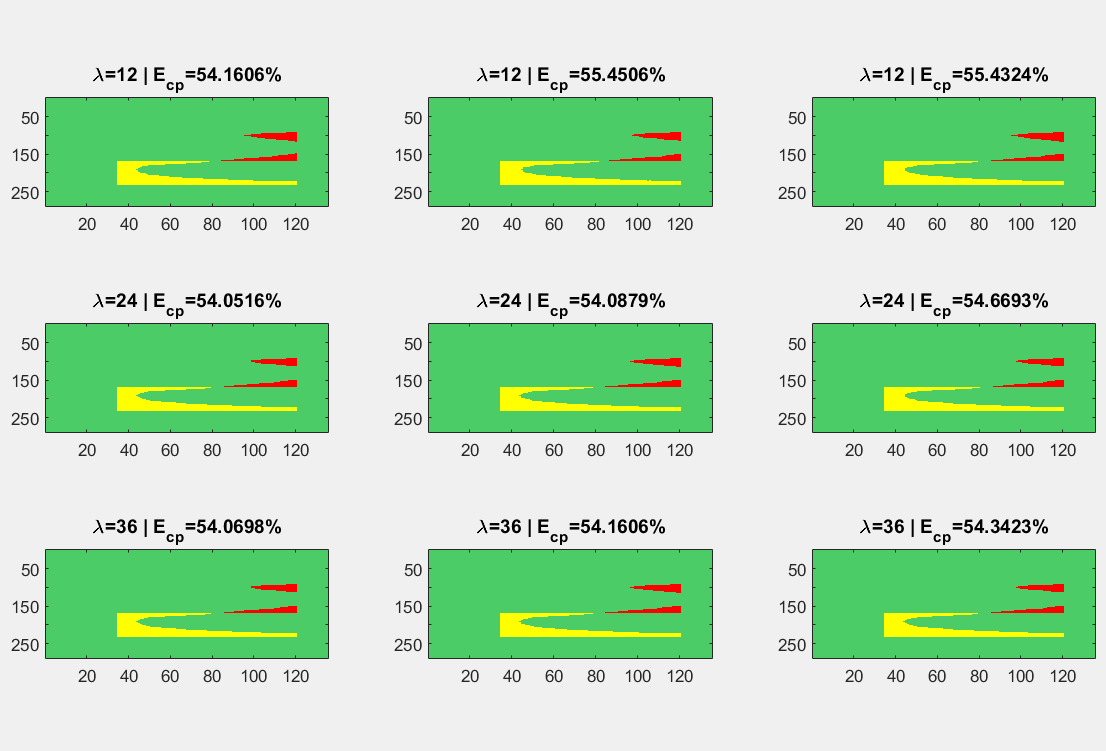
\includegraphics[width=4.5in]{figures/results_figures/lambda/cp_lambda_all.png}
	\end{figure}
\end{frame}

\begin{frame}
	\frametitle{Experiment results}
	\framesubtitle{Effects of $\lambda$}
	\begin{figure}
		\centering
		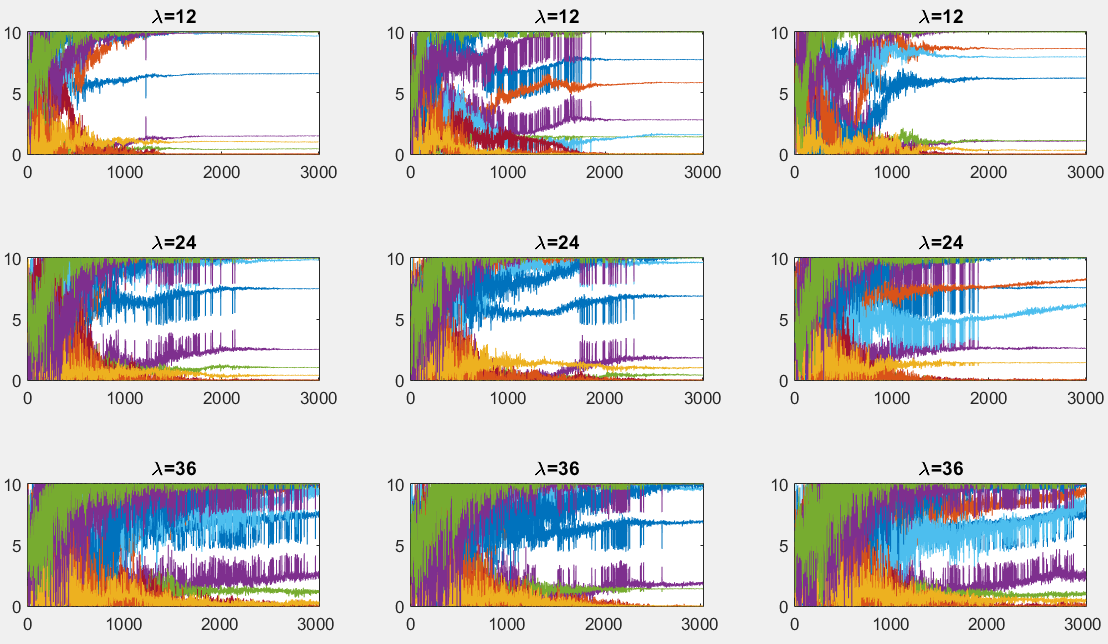
\includegraphics[width=4.5in]{figures/results_figures/lambda/knobs_lambda_all.png}
	\end{figure}
\end{frame}

\begin{frame}
	\frametitle{Experiment results}
	\framesubtitle{Effects of $\lambda$}
	\begin{figure}
		\centering
		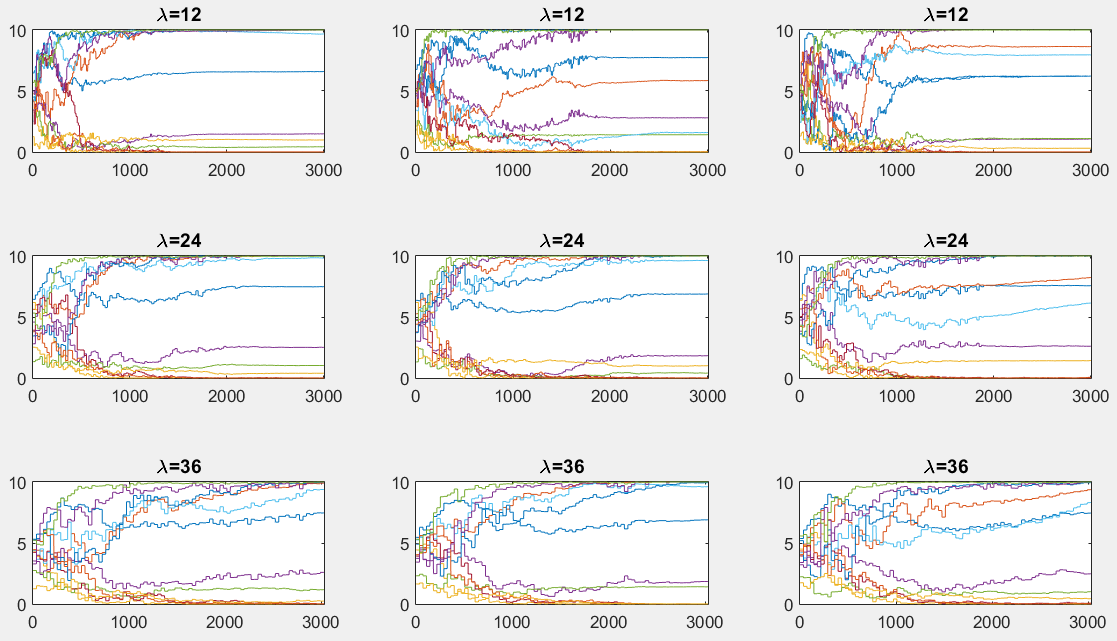
\includegraphics[width=4.5in]{figures/results_figures/lambda/knobs_lambda_all_genmean.png}
	\end{figure}
\end{frame}


\begin{frame}
	\frametitle{Further work}
	\framesubtitle{Next steps and ideas}
	\begin{itemize}
		\item Modulate the templates shapes
		\item More accurate knob boundaries
		\item New constraints/objectives
		\item MO-CMAES
		\item Parallelization
		\item Wider loop with fundamental diagrams
	\end{itemize}
\end{frame}



\end{document}